\documentclass[11pt, italian, openany]{book}
% Set page margins
\usepackage[margin=2cm]{geometry}

\usepackage[]{graphicx}
\usepackage{setspace}
\usepackage{fontspec}
\usepackage{amsmath}
\usepackage{amssymb}
\setmainfont{TeX Gyre Termes}
\singlespace % interlinea singola

\usepackage{hyperref}
\hypersetup{
	colorlinks=true,
	linkcolor=blue,
	filecolor=magenta,
	urlcolor=blue,
}
 
% All page numbers positioned at the bottom of the page
\usepackage{fancyhdr}
\usepackage{algorithmicx}
\usepackage{algpseudocode}
\fancyhf{} % clear all header and footers
\fancyfoot[C]{\thepage}
\renewcommand{\headrulewidth}{0pt} % remove the header rule
\pagestyle{fancy}

% Changes the style of chapter headings
\usepackage{titlesec}

\titleformat{\chapter}
   {\normalfont\LARGE\bfseries}{\thechapter.}{1em}{}

% Change distance between chapter header and text
\titlespacing{\chapter}{0pt}{35pt}{\baselineskip}
\usepackage{titlesec}
\titleformat{\section}
	[hang] % \textlessshape\textgreater
	{\normalfont\bfseries\Large} % \textlessformat\textgreater
	{} % \textlesslabel\textgreater
	{0pt} % \textlesssep\textgreater
	{} % \textlessbefore code\textgreater
\renewcommand{\thesection}{} % Remove section references...
\renewcommand{\thesection}{\arabic{section}} %... from sections
\usepackage{titlesec}

\setcounter{tocdepth}{5}
\setcounter{secnumdepth}{5}

% Prevents LaTeX from filling out a page to the bottom
\raggedbottom

\usepackage{color}
\usepackage{xcolor}
\usepackage{enumitem}
\usepackage{amsmath}
\usepackage{subcaption}
% Code Listings
\definecolor{vgreen}{RGB}{104,180,104}
\definecolor{vblue}{RGB}{49,49,255}
\definecolor{vorange}{RGB}{255,143,102}
\definecolor{vlightgrey}{RGB}{245,245,245}

\definecolor{codegreen}{rgb}{0,0.6,0}
\definecolor{codegray}{rgb}{0.5,0.5,0.5}
\definecolor{codepurple}{rgb}{0.58,0,0.82}
\definecolor{backcolour}{rgb}{0.95,0.95,0.92}

\usepackage{listings}

\lstdefinestyle{code}{
	language=bash,
	backgroundcolor=\color{backcolour},
	commentstyle=\color{codegreen},
	keywordstyle=\color{magenta},
	numberstyle=\tiny\color{codegray},
	stringstyle=\color{codepurple},
	basicstyle=\ttfamily\footnotesize,
	breakatwhitespace=false,
	breaklines=true,
	captionpos=b,
	keepspaces=true,
	numbers=left,
	numbersep=5pt,
	showspaces=false,
	showstringspaces=false,
	showtabs=false,
	tabsize=2
}

\renewcommand*\contentsname{Indice.}
\renewcommand{\figurename}{Figura}
\renewcommand{\listfigurename}{Elenco delle figure.}
\begin{document}
\begin{sloppypar}
\begin{titlepage}
	\clearpage\thispagestyle{empty}
	\centering
	\vspace{1cm}

	
\includegraphics[scale=0.60]{images/unipi-logo.png}

	{\normalsize \noindent Dipartimento di Informatica \\
			Corso di Laurea in Informatica \par}
	
	\vspace{2cm}
	{\Huge \textbf{Reti di Calcolatori} \par }

	\vspace{4cm}

	{\normalsize Giacomo Trapani \\ Anno Accademico 2021/2022\par}

	\pagebreak

\end{titlepage}
\tableofcontents
\listoffigures
\pagebreak
\section*{Premessa.}
Si danno le seguenti definizioni:
\begin{itemize}[topsep=0pt, itemsep=0pt, parsep=0pt]
	\item \textbf{Rete}: interconnessione di dispositivi in grado di scambiarsi informazioni, quali sistemi terminali, router, switch e modem.
	\item \textbf{Host} (\textbf{sistema terminale}): sono macchine appartenenti agli utenti finali, dedicate all'esecuzione di applicazioni (e.g. computer,
	tablet, smartphone) oppure ``server" che forniscono servizi a diverse applicazioni utente (e.g. posta elettronica, web).
	\item \textbf{Dispositivi di interconnessione}: si distinguono in ``router" (i.e. dispositivi che interconnettono reti) e ``switch"
	(i.e. dispositivi che collegano fra loro molteplici host a livello locale).
	\item \textbf{Collegamenti} (\textbf{link}): mezzi trasmissivi (cablati, wireless).
\end{itemize}
\section{Tipi di Reti.}
\subsection{LAN (Local Area Network).}
Le LAN vengono definite come reti di computer circoscritte a un'area geograficamente limitata (si estendono al pi\`u per alcuni chilometri,
sono circoscritte ad aree limitate come un ufficio, una scuola, un edificio etc.). Si cita Ethernet come tecnologia LAN popolare.

Le LAN sono tipicamente di propriet\`a di una qualche organizzazione (sono dunque reti private), connettono sistemi terminali (stampanti, PC,
workstations) mediante cavi di rame o connessioni wireless.

Si distinguono LAN con cavo condiviso (obsolete) e LAN con switch (moderne); il maggiore vantaggio della seconda sulla prima \`e che non ha
bisogno di far passare un pacchetto da ogni dispositivo connesso nel percorso dal router al (dispositivo) target.

Si veda la figura \ref{fig:LAN}.

\subsection{WAN (Wide Area Network).}
Una WAN (o rete geografica) \`e una rete il cui compito \`e di interconnettere LAN o singoli host separati da distanze geografiche. Viene
tipicamente gestita da un operatore di rete che fornisce servizi ai clienti. Un esempio di WAN \`e la rete GARR.

Si distinguono WAN punto-punto (collegano direttamente due dispositivi attraverso un mezzo trasmissivo (e.g. cavo in fibra ottica, ponti radio))
e WAN a commutazione (collegano pi\`u di due punti di terminazioni (e.g. dorsali Internet)); le seconde sono dotate di elementi di commutazione
(i.e. elaboratori specializzati utilizzati per connettere tra loro pi\`u linee di trasmissione).

Si veda la figura \ref{fig:WAN}.

\section{Tecniche di commutazione.}
Si definiscono ``tecniche di commutazione" le modalit\`a con cui viene determinato il percorso sorgente-destinazione e vengono dedicate ad esso le
risorse della rete. Si distinguono due tecniche: circuit switching (si parla di ``reti a commutazione di circuito") e packet switching (``reti a
commutazione di pacchetto").

Si veda la figura \ref{fig:tipi-reti}.

\subsection{Circuit switching.}
La rete determina un percorso dalla sorgente alla destinazione, su questo viene riservato e garantito un rate di trasmissione costante per la
durata dell'intera sessione di comunicazione (una frazione della capacit\`a di trasmissione dei link).

Un esempio di rete a commutazione \`e la rete telefonica fissa tradizionale.

\textbf{Svantaggi}: le risorse rimangono inattive quando non utilizzate e non vengono mai condivise, necessaria una fase di instaurazione della
comunicazione (detta anche di ``setup") nella quale si configurano le tabelle di switching, la scarsa flessibilit\`a nell'uso delle risorse pu\`o
portare a ``overprovisioning" e/o a un sottoutilizzo di queste in presenza di rate di traffico variabile.

\textbf{Vantaggi}: performance garantita, overhead limitato, tecnologie di switching efficienti.

\subsection{Packet switching.}
Il flusso di dati punto-punto viene suddiviso in pacchetti che condividono le risorse di rete e instradati singolarmente e indipendentemente
dagli altri. Si parla di trasmissione ``store and forward": il commutatore (tipicamente un router) deve aspettare di aver ricevuto per intero il
pacchetto prima di poter trasmettere sul collegamento in uscita.

Non c’\`e un canale dedicato e la sequenza dei pacchetti non segue uno schema prestabilito (si parla di ``multiplexing statistico"): i router
possono memorizzare i pacchetti nelle code (``buffer") nel caso in cui il collegamento sia gi\`a usato alla massima capacit\`a, introducendo
dunque dei ``ritardi di coda" e il rischio di ``congestione"; non si ha garanzia nelle prestazioni e si corre il rischio di avere una perdita
di pacchetti poich\'e i buffer hanno dimensione finita.

\textbf{Svantaggi}: alto overhead, tecnologie di inoltro non efficienti (si ha la necessit\`a di selezionare l’uscita per ogni pacchetto),
tempo di elaborazione ai router (si parla di ``routing table lookup"), accodamento ai router.

\textbf{Vantaggi}: risorse trasmissive usate solo su richiesta, segnalazione non necessaria.

\section{Internet.}
Si definisce ``internet" una rete costituita da due o pi\`u reti interconnesse; un esempio di internet \`e Internet, una rete a commutazione di
pacchetti composta da migliaia di reti interconnesse che seguono l'Internet Protocol e rispettano convenzioni precise per nomi e indirizzi, che
fornisce servizi di comunicazione alle applicazioni e per le applicazioni.

Le reti dei sistemi terminali sono connesse a Internet attraverso una gerarchia di fornitori di servizi internet (Internet Service Provider);
definisco ``dorsale" una ISP di primo livello. Si permette l'esistenza di ``Internet eXchange Point", definiti come punti di incontro per il peering
tra due o pi\`u ISP.

Si veda la figura \ref{fig:internet}.

\subsection{Metriche.}
Si definiscono i seguenti parametri, utilizzati per misurare le prestazioni della rete:
\begin{itemize}[topsep=0pt, itemsep=0pt, parsep=0pt]
	\item \textbf{Larghezza di banda} (\textbf{Bandwidth}): larghezza dell’intervallo di frequenze utilizzato dal sistema trasmissivo misurato in Hertz.
	\item \textbf{Velocit\`a di trasmissione} (\textbf{Bitrate o transmission rate}): quantit\`a di dati (bits) che possono essere trasmessi (“inseriti
	nella linea”) nell'unit\`a di tempo (bits/secondo o bps) su un certo collegamento; dipende alla larghezza di banda e dalla tecnica trasmissiva
	utilizzata.
	\item \textbf{Throughput}: quantit\`a di dati che possono essere trasmessi da un nodo sorgente a un nodo destinazione in un certo intervallo di tempo
	al netto di perdite sulla rete, duplicazioni, protocolli etc.
	\item \textbf{Latenza}: tempo richiesto affinch\'e un messaggio arrivi a destinazione dal momento in cui il primo bit parte dalla sorgente; \`e
	definito come somma di ritardo di elaborazione, di accodamento, di trasmissione e di propagazione.
\end{itemize}
Si definiscono dunque i ritardi sopra elencati:
\begin{itemize}[topsep=0pt, itemsep=0pt, parsep=0pt]
	\item \textbf{Ritardo di elaborazione}: \`e dovuto al controllo di errori sui bit e alla determinazione del canale di uscita.
	\item \textbf{Ritardo di accodamento}: \`e il tempo che un pacchetto spende all'interno del buffer (tipicamente di un router), \`e una
	quantit\`a aleatoria.
	\item \textbf{Ritardo di trasmissione}: \`e il tempo impiegato per trasmettere un pacchetto sul link; definendo L lunghezza del pacchetto in bit,
	R rate di trasmissione sul link in bps, vale \( \frac{L}{R} \).
	\item \textbf{Ritardo di propagazione}: \`e il tempo che 1bit impiega per essere propagato da un nodo all'altro; definendo d lunghezza del
	collegamento fisico, s velocit\`a di propagazione nel mezzo, vale \( \frac{d}{s} \).
\end{itemize}
Si definisce inoltre il ``ritardo end-to-end" come sommatoria del ritardo ai singoli nodi: \\\( R_{end-to-end} = \sum_{i=1}^{N} R_{nodo_i}\).

Si ricorda l'esistenza dei comandi ``traceroute", che traccia un pacchetto dal proprio dispositivo all'host mostrando anche il numero di passaggi
(salti) necessari per raggiungerlo assieme al ritardo dal mittente per ogni passaggio (nello specifico, usa il protocollo UDP per inviare datagrammi
configurati in modo tale da scatenare messaggi di errore dovuti a ``tempo scaduto" o ``porta destinazione non raggiungibile''),
e ``ping", che calcola il ritardo per la trasmissione dal dispositivo corrente all'host.

\section{Modelli stratificati.}
Si definisce un ``protocollo" un insieme di regole che permettono a due entit\`a di comunicare; nei sistemi di comunicazione non \`e
sufficiente un singolo protocollo, si ricorre a una organizzazione di protocolli.

Si definisce inoltre ``aperto" un insieme di protocolli i cui dettagli sono disponibili pubblicamente e i cui cambiamenti sono gestiti da una
organizzazione la cui partecipazione \`e aperta al pubblico; definisco "sistema aperto" un sistema che implementa protocolli aperti.

Per la stratificazione si fa riferimento ai principi di ``separation of concern" (i.e. separazione degli interessi e delle responsabilit\`a, fare
ci\`o che compete, delegando ad altri tutto ci\`o che \`e delegabile) e ``information hiding" (i.e. nascondere tutte le informazioni che non sono
indispensabili per il committente per definire completamente un'operazione).

In concreto:
\begin{itemize}[topsep=0pt, itemsep=0pt, parsep=0pt]
	\item Il modello permette di scomporre il problema in sottoproblemi pi\`u semplici il cui sviluppo \`e indipendente (da quello degli altri
	sottoproblemi).
	\item Ogni strato scambia informazioni con quelli adiacenti, ma comunica logicamente con il proprio omologo; fornisce informazioni allo strato
	superiore e usa i servizi offerti da quello inferiore.
	\item Un singolo strato svolge una sola funzione e realizza uno e un solo livello logico.
\end{itemize}

A questo punto l'obiettivo diventa realizzare una rete di calcolatori in cui qualsiasi terminale comunica con un qualsiasi fornitore di servizi
mediante qualsiasi rete; lo standard per l'interconnessione di sistemi aperti \`e il modello ISO/OSI.

\subsection{Modello ISO/OSI.}
Si danno le seguenti definizioni nei termini del modello ISO/OSI:
\begin{itemize}[topsep=0pt, itemsep=0pt, parsep=0pt]
	\item \textbf{Livello} (o \textbf{strato}): modulo interamente definito attraverso i servizi, protocolli e le interfacce che lo caratterizzano.
	\item \textbf{Servizio}: insieme di primitive (operazioni) che uno strato fornisce ad uno strato soprastante.
	\item \textbf{Interfaccia}: insieme di regole che governano il formato e il significato delle unit\`a di dati (es. messaggi, segmenti o
	pacchetti) che vengono scambiati tra due strati adiacenti della stessa entit\`a.
	\item \textbf{Protocollo}: insieme di regole che permettono a due entit\`a omologhe (stesso strato) uno scambio efficace ed efficiente delle
	informazioni, definiscono il formato e l’ordine dei messaggi inviati e ricevuti tra entit\`a omologhe della rete e le azioni che vengono
	fatte per la trasmissione e ricezione dei messaggi; occorre specificare sintassi e semantica di un messaggio e quali azioni intraprendere
	una volta ricevuto.
\end{itemize}

Per uno schema, si veda la figura \ref{fig:iso-osi}.

I layer dal livello 5 al 7 sono di supporto all'elaborazione e interazione con l'utente (vengono realizzati a livello software), gli altri 4
alla rete e all'infrastruttura trasmissiva (realizzati a livello hardware e software); tipicamente i nodi intermedi implementano solo i primi
4.

Il modello prevede inoltre l'incapsulamento: il flusso di informazioni - che ha origine al livello applicativo - discende verso i livelli inferiori e
viene progressivamente arricchito mediante l'aggiunta di headers.

Si danno in proposito le seguenti definizioni:
\begin{itemize}[topsep=0pt, itemsep=0pt, parsep=0pt]
	\item \textbf{Header}: qualificazione del pacchetto dati al livello corrente.
	\item \textbf{Data}: payload proveniente dal livello precedente.
	\item \textbf{Trailer}: usato in funzione di trattamento dell'errore.
\end{itemize}

\subsection{Stack protocollare TCP/IP.}
TCP/IP \`e una famiglia di protocolli attualmente utilizzata in Internet. Si tratta di una gerarchia di protocolli, ciascuno dei quali fornisce
funzionalit\`a specifiche. Prende di riferimento il modello ISO/OSI e si articola nei seguenti 5 livelli (elencati dall'alto al basso):
\begin{itemize}[topsep=0pt, itemsep=0pt, parsep=0pt]
	\item \textbf{Application Layer}: \`e di supporto alle applicazioni di rete, permette un collegamento logico end-to-end; si usa per lo scambio di
	pacchetti di informazioni detti ``messaggi". Include i protocolli HTTP, FTP, SMTP...
	\item \textbf{Transport Layer}: permette il trasporto di messaggi tra sistemi terminali; un pacchetto a questo livello prende il nome di ``segmento".
	Include i protocolli TCP (connection oriented, garantisce la consegna dei messaggi) e UDP (connectionless, non garantisce la consegna dei messaggi).
	\item \textbf{Network Layer}: si occupa dell'instradamento di pacchetti detti ``datagrammi" dalla sorgente alla destinazione tipicamente attraversando
	una serie di router. Include i protocolli IP, ICMP.
	\item \textbf{Link Layer}: si occupa di trasferire pacchetti detti ``frame" attraverso il collegamento tra elementi di rete vicini. Include i protocolli
	Ethernet, PPP, WiFi...
	\item \textbf{Physical Layer}: si occupa di trasferire individualmente i bit contenuti nei singoli frame da un nodo al successivo.
\end{itemize}

Si veda la figura \ref{fig:comunicazione-internet}.

\subsubsection{Application Layer.}
Si danno in merito le seguenti definizioni:
\begin{itemize}[topsep=0pt, itemsep=0pt, parsep=0pt]
	\item \textbf{Application Programming Interface}: insieme di regole che un programmatore deve rispettare per l'utilizzo delle risorse.
	\item \textbf{Socket}: API che funge da interfaccia tra gli application e transport layer; due processi comunicano mandando dati alla socket (che
	fa da connessione a livello logico) il cui invio e ricezione sono responsabilit\`a dei restanti quattro livelli dello stack TCP/IP nel sistema
	operativo. \`E la API di Internet.
	\item \textbf{Uniform Resource Identifier}: stringa di caratteri che identifica una risorsa (i.e. qualsiasi cosa abbia una identit\`a) presente
	sulla rete. Se ne distinguono di due tipi:
	\begin{itemize}[topsep=0pt, itemsep=0pt, parsep=0pt]
		\item \textbf{Uniform Resource Locator}: sottoinsieme di URI che identifica le risorse attraverso il loro meccanismo di accesso. Segue la sintassi
		\textless{scheme}\textgreater{://}\textless{user}\textgreater{:}\textless{password}\textgreater{@}\textless{host}\textgreater{:}\textless{port}
		\textgreater{/}\textless{path}\textgreater:
		``scheme" identifica il protocollo, ``user" e ``password" sono opzionali e generalmente deprecati, ``host" \`e il nome di dominio di un host,
		``port" \`e il numero di porta del server, ``path" identifica la risorsa nel contesto specificato.
		\item \textbf{Uniform Resource Name}: sottoinsieme di URI che devono rimanere globalmente unici e persistente anche quando la risorsa cessa di
		esistere e diventa non disponibile.
	\end{itemize}
\end{itemize}

A questo livello si distinguono due modelli architetturali:
\begin{itemize}[topsep=0pt, itemsep=0pt, parsep=0pt]
	\item \textbf{Client-Server}: esiste un host sempre attivo (il ``server") che serve le richieste di altri host (i ``clients").
	\item \textbf{Peer-to-Peer}: la comunicazione avviene tra coppie di dispositivi non sempre attivi (i ``peer") che possono offrire servizi e inviare
	richieste.
\end{itemize}

Per poter inviare dati risulta necessario poter indirizzare opportunamente il processo destinatario: per Internet si usa la coppia indirizzo IP (i.e. un
intero a 32bit che identifica univocamente una macchina host), numero di porta (un intero a 16bit che identifica univocamente un processo all'interno di
una macchina).

Il livello di trasporto mette a disposizione due protocolli diversi per la comunicazione:
\begin{itemize}[topsep=0pt, itemsep=0pt, parsep=0pt]
	\item \textbf{TCP}: ha le seguenti caratteristiche:
	\begin{itemize}[topsep=0pt, itemsep=0pt, parsep=0pt]
		\item \textbf{Connection-oriented}: \`e necessaria una fase di setup iniziale tra client e server prima di poter trasmettere messaggi (si parla
		di ``handshaking").
		\item \textbf{Controllo del flusso}: il mittente non ``inonder\`a" di dati il destinatario.
		\item \textbf{Controllo di congestione}: ``strangola" il mittente (client o server) quando la rete \`e sovraccarica.
		\item Garantisce il trasporto affidabile tra processo mittente e destinatario.
		\item Non offre garanzie di timing n\'e di ampiezza minima di banda.
	\end{itemize}
	\item \textbf{UDP}: ha le seguenti caratteristiche:
	\begin{itemize}[topsep=0pt, itemsep=0pt, parsep=0pt]
		\item \textbf{Connectionless}: non orientato alle connessioni, non prevede una fase di setup iniziale.
		\item Trasporto non affidabile.
		\item Non implementa meccanismi di controllo di flusso.
		\item Non implementa meccanismi per il controllo di congestione.
		\item Non offre garanzie di timing n\'e ampiezza minima di banda.
	\end{itemize}
\end{itemize}

Per degli esempi di applicazioni Internet, si veda la figura \ref{fig:applicazioni-internet}.

Si passa dunque alla trattazione dei protocolli implementati a questo livello:
\begin{itemize}[topsep=0pt, itemsep=0pt, parsep=0pt]
	\item \textbf{HTTP}: ha le seguenti caratteristiche:
	\phantomsection
	\addcontentsline{toc}{paragraph}{HTTP}
	\begin{itemize}[topsep=0pt, itemsep=0pt, parsep=0pt]
		\item \textbf{Stateless}: non ha memoria di stato: le coppie richiesta, risposta sono indipendenti; ogni richiesta viene eseguita indipendentemente
		da quelle che la han preceduta.
		\item \textbf{Richiesta/Risposta}: La connessione viene iniziata dal client, che invia un messaggio di richiesta detto ``request" a cui il server
		risponde con un messaggio di risposta detto ``response".
		\item \textbf{Content negotiation}: permette di selezionare la rappresentazione appropriata per una risorsa (e.g. formato, lingua etc) quando
		viene servita richiesta.
		\item \textbf{Web caching}: si memorizzano copie temporanee di risorse Web (es. pagine HTML, immagini) e vengono servite al client per ridurre
		l’uso di risorse (e.g. banda, workload sul server) e il tempo di risposta al client.
		\item Implementa i ``cookie": un pacchetto di informazioni assegnato dal server alla prima richiesta del client che, a sua volta, lo legge dal
		messaggio di risposta (in cui trova una linea ``set-cookie") e lo salva in un file; il cookie viene poi aggiunto dal client a tutte le successive
		richieste a quel sito (conterranno la linea ``cookie:\textless{cookie}\textgreater{)}".
		\item Usa TCP.
		\item HTTP/1.0 permetteva solo connessioni non persistenti, HTTP/1.1 prevede che - di default - le connessioni siano invece persistenti e vengano
		mantenute fino a una richiesta di chiusura. I server che rispettano HTTP/1.1 supportano inoltre il pipelining (i.e. consiste nell’invio da parte del
		client di molteplici richieste senza aspettare la ricezione di ciascuna risposta, il server deve inviare le risposte nello stesso ordine in cui
		sono state ricevute; riguarda solo metodi idempotenti); implementato in pochi browser, introduce il rischio di Head of Line Blocking (i.e. se una
		richiesta richiede tempo per essere processata le risposte a quelle successive sono bloccate).
	\end{itemize}

	Per la struttura dei messaggi HTTP, si veda la figura \ref{fig:messaggi-http}.

	I metodi messi a disposizione dal protocollo sono:
	\begin{itemize}[topsep=0pt, itemsep=0pt, parsep=0pt]
		\item \textbf{OPTIONS}: richiede informazioni sulle opzioni di comunicazione (i.e. quali metodi) sono associati a una URL o al server stesso.
		\item \textbf{GET}: richiede il trasferimento di una risorsa identificata da una URL o operazioni associate all’URL stessa; la semantica pu\`o
		essere modificata in un ``conditional GET" se l'header contiene uno dei campi ``If-Modified-Since", ``If-Unmodified-Since", ``If-Match",
		``If-None-Match" o ``If-Range", ``partial GET" se contiene il campo ``range".
		\item \textbf{HEAD}: identico al metodo GET con l'eccezione che la risposta non contiene il campo ``message-body".
		\item \textbf{POST}: serve per inviare dal client al server informazioni inserite nel body del messaggio, la funzione effettiva determinata \`e
		dal server e dipendente tipicamente dalla Request-URI; tipicamente non \`e abilitato sui server pubblici.
		\item \textbf{PUT}: il client chiede al server di creare/modificare una risorsa.
		\item \textbf{DELETE}: il client chiede di cancellare una risorsa.
		\item TRACE.
	\end{itemize}

	Si definiscono ``safe" i metodi che non modificano la rappresentazione di una risorsa (i.e. GET, HEAD, OPTIONS, TRACE), ``idempotent" quelli che godono
	della propriet\`a di idempotenza (i.e. GET, HEAD, PUT, DELETE, OPTIONS, TRACE).

	\item \textbf{TErminaL NETwork}: ha le seguenti caratteristiche
	\addcontentsline{toc}{paragraph}{TELNET}
	\begin{itemize}[topsep=0pt, itemsep=0pt, parsep=0pt]
		\item Prevede un programma server che accetta le richieste e un programma client che effettua le richieste; quest'ultimo interagisce con il terminale
		utente sull'host locale e scambia messaggi con il Telnet server.
		\item Usa TCP e persiste per l'intera durata della sessione, il client si connette alla porta 23 del server.
		\item Il client accetta le battute di tasti del terminale e le invia al server nel quale un software chiamato ``pseudo terminal driver" fa da entry
		point del sistema operativo: consente di trasferire caratteri a un processo come se provenissero dal terminale.
		Il client accetta i caratteri che il server manda indietro e li visualizza sul terminale utente.
		\item  I messaggi di controllo iniziali sono usati per scambiare informazioni sulle caratteristiche degli host (si parla di ``Telnet option
		negotiation").
		\item Il client invia (in chiaro) un login identifier e una password (non \`e sicuro, \`e stato sostituito da ``SSH").
	\end{itemize}

	Il terminale in esecuzione sia sul client sia sul server \`e un ``Network Virtual Terminal": gli host traducono le loro caratteristiche locali cos\`i da
	apparire esternamente come un NVT e assumono che l’host remoto sia un NVT; si scambiano dati e comandi in formato 7-bit US-ASCII sullo stesso canale
	(prevede dunque ``in-band signaling"), ogni carattere \`e inviato come un ottetto con il primo bit settato a 0 se si tratta di un dato, a 1 per i comandi.

	Si veda la figura \ref{fig:telnet}.

	\item \textbf{Simple Mail Transfer Protocol}: si danno in merito le seguenti definizioni:
	\addcontentsline{toc}{paragraph}{SMTP}
	\begin{itemize}[topsep=0pt, itemsep=0pt, parsep=0pt]
		\item \textbf{User agent}: componente che permette l'invio, la modifica e la lettura di messaggi di posta elettronica.
		\item \textbf{Mail server}: componente che trasferisce i messaggi di posta elettronica.
		\item \textbf{Indirizzo email}: stringa che identifica un destinario, ha la struttura
		``\textless{local-part}\textgreater{@}\textless{domain-name}\textgreater{"}:
		la prima parte identifica il destinatario all'interno del mail server, la seconda (identifica) il mail server.
		\item \textbf{Tipo MIME}: specifica la natura dei dati nel corpo di un'entit\`a MIME.
	\end{itemize}

	Il protocollo ha le seguenti caratteristiche:
	\begin{itemize}[topsep=0pt, itemsep=0pt, parsep=0pt]
		\item Ha come obiettivo \textbf{trasferimento affidabile ed efficiente di email}.
		\item Implementa un meccanismo di \textbf{scambio formale di responsabilit\`a}: i client hanno come responsabilit\`a trasferire email a un server SMTP o
		comunicare un eventuale insuccesso.
		\item \`E indipendente dal sistema di trasmissione usato e richiede solo il \textbf{trasferimento di stream di byte ordinato e affidabile} (tipicamente,
		si usano connessioni TCP su porta 25).
		\item Ha la capacit\`a di \textbf{trasportare mail attraverso pi\`u reti} (i.e. un messaggio di mail può passare attraverso server intermedi nel
		percorso da mittente a destinatario finale).
		\item I messaggi sono costituiti da una componente \textbf{header} (i.e. linee di intestazione, tra cui ``To:'', ``From'', ``Subject'') e un
		\textbf{body} (i.e. il corpo del messaggio formato da soli caratteri ASCII 7bit).
		\item Le interazioni tra client e server sono del tipo \textbf{command}/\textbf{response}: a ogni comando (testo ASCII 7 bit) corrisponde una risposta
		formata da codice di stato e opzionalmente una descrizione.
		\item \`E un protocollo di tipo \textbf{push}.
	\end{itemize}

	I mail server implementano una tecnica denominata ``spooling": al momento dell'invio di un messaggio, il sistema (client) copia messaggio, identificativo
	del mittente, del destinatario e della macchina di destinazione e tempo di deposito in un'area di memoria detta ``spool"; il client stabilisce una
	connessione TCP con la macchina destinazione, se questo ha successo allora la copia locale viene eliminata; il processo di trasferimento scandisce
	periodicamente lo spool ed esegue la procedura di trasferimento dei messaggi non consegnati, dopo un intervallo di tempo definito dall'amministratore del
	server se un messaggio non \`e stato ancora consegnato allora l'utente mittente viene notificato.

	Si veda la figura \ref{fig:smtp}.

	Si identificano tre fasi per il trasferimento SMTP:
	\begin{itemize}[topsep=0pt, itemsep=0pt, parsep=0pt]
		\item \textbf{Handshaking}: nella fase di setup iniziale, il client stabilisce la connessione e attende dal server il messaggio di risposta
		``220 READY FOR MAIL", che indica la disponibilit\`a a ricevere posta.
		\item \textbf{Trasferimento del messaggio}.
		\item \textbf{Chiusura della connessione}.
	\end{itemize}

	I mail server moderni permettono la negoziazione per l'invio di dati in codifica binaria (quindi a 8bit), se non ha successo si inviano caratteri ASCII 7bit
	seguendo il \textbf{protocollo MIME}. MIME fornisce regole di codifica e decodifica per trasformare caratteri speciali e contenuti multimediali in caratteri
	ASCII 7bit (in questo modo, si garantisce la retrocompatibilit\`a con i mail server e non con gli user agent), permette inoltre l'uso di pi\`u codifiche
	all'interno dello stesso messaggio con il tipo ``multipart'', che specifica il ``boundary'' (confine) tra ciascuna.

	Per indicare la fine di un messaggio si usa la seguenza di caratteri ``\textless{CLRF}\textgreater{.}\textless{CLRF}\textgreater{"}. Vengono messi a
	disposizione i seguenti comandi:
	\begin{itemize}[topsep=0pt, itemsep=0pt, parsep=0pt]
		\item \textbf{HELO} \textless{client identifier}\textgreater{;}
		\item \textbf{MAIL FROM:}\textless{\textbf{reverse-path}\textgreater{\textless{CRLF}\textgreater{;}}}
		\item \textbf{RCPT TO:}\textless{\textbf{forward-path}\textgreater{CRLF\textgreater{;}}}
		\item \textbf{DATA};
		\item \textbf{QUIT}.
	\end{itemize}

	Si veda la figura \ref{fig:smtp-esempi}.

	SMTP \`e un protocollo di tipo ``push", per la ricezione risulta necessario un protocollo di tipo ``pull". Alcuni esempi sono: Post Office Protocol
	(\textbf{POP}), Internet Mail Access Protocol (\textbf{IMAP}), \textbf{HTTP} (quando user agent \`e un browser).

	\item \textbf{Domain Name Server}: si danno in merito le seguenti definizioni:
	\addcontentsline{toc}{paragraph}{DNS}
	\begin{itemize}[topsep=0pt, itemsep=0pt, parsep=0pt]
		\item \textbf{Nome}: identifica un oggetto con una sequenza di caratteri scelti da un alfabeto finito; si usa per motivi mnemonici e per disaccoppiare
		il livello applicativo da quello di rete.
		\item \textbf{Indirizzo}: identifica la locazione dell'oggetto (i dispositivi connessi alla rete vengono individuati mediante indirizzi da 4byte detti
		``indirizzi IP").
		\item \textbf{Dominio}: sottoalbero nello spazio dei nomi di dominio che viene identificato dal nome di dominio del nodo in cima al sottoalbero.
		\item \textbf{Sottodomini}: insieme dei domini in cui si pu\`o suddividere un dominio.
		\item \textbf{Name server}: programma che gestisce la conversione da nome di dominio a indirizzo IP.
	\end{itemize}


	DNS offre i seguenti servizi:
	\begin{itemize}[topsep=0pt, itemsep=0pt, parsep=0pt]
		\item \textbf{Risoluzione di nomi} di alto livello (``hostname") in indirizzi IP.
		\item \textbf{Host aliasing}: un host può avere più nomi, vengono tradotti nel nome canonico e - di seguito - nell'indirizzo IP.
		\item \textbf{Mail server aliasing}: sinonimi per mail server; e.g. nome identico per mail server e web server).
		\item \textbf{Distribuzione carico}: un hostname canonico può corrispondere a più indirizzi IP, il DNS restituisce la lista variandone l'ordine per
		ogni risposta.
	\end{itemize}

	Concretamente, DNS \`e costituito da:
	\begin{itemize}[topsep=0pt, itemsep=0pt, parsep=0pt]
		\item \textbf{Schema di assegnazione dei nomi} gerarchico e basato su domini.
		\item \textbf{Database distribuito} contenente i nomi e le corrispondenze con gli indirizzi IP implementato con una gerarchia di name server (``record
		DNS'').
		\item \textbf{Protocollo per la distribuzione delle informazioni sui nomi tra name server}: host, router, name server comunicano per risolvere nomi
		(traduzione nome/indirizzo) utilizzando tipicamente UDP con porta 53.
	\end{itemize}

	Si vedano le figure \ref{fig:dns-servizio} e \ref{fig:dns-nameserver}.

	A livello pratico, garantire una struttura gerarchica per i nomi permette di delegarne l'assegnazione a singoli organizzazioni e distribuire la conversione
	di nomi e indirizzi.

	Lo spazio dei domini ha una struttura ad albero; ogni nodo dell'albero ha un \textbf{nome di dominio}, ossia una sequenza di diverse
	etichette (i.e. stringhe) separate da punti (e.g. ``lab3''.``di''.``unipi''.``it''). Inoltre, si definisce \textbf{zona} la regione (tipicamente una parte
	contigua dell’albero) di cui \`e responsabile un name server; per esempio, in ``di.unipi.it'' zona e dominio coincidono, lo stesso discorso non vale per 
	``unipi.it''.

	Per esempi di query DNS, si veda la figura \ref{fig:dns-query}.

	Si distinguono i seguenti ruoli:
	\begin{itemize}[topsep=0pt, itemsep=0pt, parsep=0pt]
		\item \textbf{Server Top-Level Domain}: mantiene le informazioni dei nomi di dominio che appartengono a un certo TLD, restituisce le informazioni
		sui name server di competenza dei sottodomini.
		\item \textbf{Server Radice}: responsabile dei record della zona radice e restituisce le informazioni sui name server di TLD.
		\item \textbf{Server di Competenza} (\textbf{Authoritative Name Server}): autorità per una certa zona, memorizza nome e indirizzo IP di un insieme di
		host dei quali può effettuare traduzioni nome/indirizzo; per una certa zona ci possono essere server di competenza primari e secondari:
		quelli primari mantengono il file di zona, quelli secondari ricevono il file di zona e offrono il servizio di risoluzione.
		\item \textbf{Local Name Servers}: non appartengono strettamente alla gerarchia dei server, ogni ISP (università, società, ISP) ha il proprio; a questi
		vengono inizialmente rivolte le query DNS: operano da proxy e inoltrano la query in una gerarchia di server DNS.
	\end{itemize}

	Spesso, i server DNS implementano al loro interno un meccanismo di caching su cui salvano dei record corrispondenti ai risultati delle query; i record
	vengono definiti come una quadrupla formata dai campi ``name", ``value", ``type", ``ttl" (time to leave).

	Dal parametro ``type" dipende il significato della coppia ``name" e ``value"; si citano alcuni esempi:
	\begin{itemize}[topsep=0pt, itemsep=0pt, parsep=0pt]
		\item \textbf{A}: ``name" sta per hostname, value per indirizzo IP.
		\item \textbf{CNAME}: ``name" sta per hostname (o un suo sinonimo), ``value" per il nome canonico dell'host.
		\item \textbf{NS}: ``name" sta per nome di dominio, ``value" per l'authorative name server per quel dominio.
		\item \textbf{MX}: ``name" sta per nome di dominio, ``value" per il nome canonico del server di posta associato a quel dominio.
	\end{itemize}

	Il protocollo DNS ha le seguenti caratteristiche:
	\begin{itemize}[topsep=0pt, itemsep=0pt, parsep=0pt]
		\item Usa connessione \textbf{UDP sulla porta 53}.
		\item \textbf{Permette} uso di \textbf{TCP} (tipicamente usata per messaggi di grandi dimensioni tra server DNS)
		\item \textbf{Messaggi di query e reply hanno lo stesso formato}. Per la struttura dei messaggi, si veda la figura \ref{fig:dns-messaggio}.
		\item Ha un \textbf{header} formato dai seguenti campi:
		\begin{itemize}[topsep=0pt, itemsep=0pt, parsep=0pt]
			\item \textbf{identification}: intero a 16bit uguale per la coppia query, reply.
			\item \textbf{flags}: 0 se query, 1 se risposta.
			\item \textbf{autorevolezza} della risposta.
		\end{itemize}
		\item \textbf{Domande}: campi per il nome richiesto e il tipo di query
		\item \textbf{Risposte}: RR nella risposta alla domanda
		\item \textbf{Competenza}: record relative ai server di competenza
		\item \textbf{Informazioni} aggiuntive
	\end{itemize}

	Essendo per natura DNS altamente centralizzato, una query attraversa una serie di server prima di restituire il risultato: in questo modo, si introduce il
	rischio di ``DNS hijacking'' (consiste nel restituire risposte non corrette alle query, si reindirizza il client verso siti malevoli). Si veda la figura
	\ref{fig:dns-hijacking}.

	Per interrogazioni a server DNS si usa il tool "dig".
	\item \textbf{File Transfer Protocol}: ha le seguenti caratteristiche:
	\addcontentsline{toc}{paragraph}{FTP}
	\begin{itemize}[topsep=0pt, itemsep=0pt, parsep=0pt]
		\item Permette control connection (i.e scambio di comandi e risposte tra client e server). Segue il protocollo Telnet.

		Il client FTP contatta il server FTP alla porta 21, ottiene l’autorizzazione sulla connessione di controllo e invia i comandi su di questa
		(e.g. cambio directory, invio file, ecc.). La connessione di controllo \`e persistente
		\item Permette data connection (i.e. connessione su cui i dati sono trasferiti con modi e tipi specificati). I dati trasferiti possono essere
		parte di un file, un file o un set di file.

		Il server apre una connessione dati TCP con il client (caveat: non \`e il client a farlo, si parla di ``modalit\`a attiva"), trasferisce il
		file sulla connessione dati e, terminata l'operazione, il server chiude la connessione. La connessione dati non \`e persistente, ne viene
		aperta e chiusa una per ciascun trasferimento.
		\item Si usa il protocollo di trasporto TCP, per cui si permettono due differenti modalit\`a: quella ``attiva" (descritta precedentemente,
		usata di default) e quella ``passiva" (in questo caso il client chiede al server di mettersi in ascolto su una porta per una connessione dati,
		ottiene questo numero di porta - tipicamente 20 - e lo usa per aprire la connessione con il server).
		\item \`E un protocollo stateful.
		\item Fa uso di codici di ritorno.
		\item Il collegamento pu\`o essere anonimo (si parla di ``anonymous FTP") o reso sicuro con TLS.
		\item Implementa pi\`u modalit\`a di trasmissione, come:
		\begin{itemize}[topsep=0pt, itemsep=0pt, parsep=0pt]
			\item \textbf{Stream mode}: FTP invia i dati a TCP con un flusso continuo di bit.
			\item \textbf{Block mode}: FTP invia i dati a TCP suddivisi in blocchi. Ogni blocco è preceduto da un header.
			\item \textbf{Compressed mode}: si trasmette il file compresso.
			\end{itemize}
	\end{itemize}

	Si veda la figura \ref{fig:ftp}.

	I comandi messi a disposizione sono i seguenti:
	\begin{itemize}[topsep=0pt, itemsep=0pt, parsep=0pt]
		\item \textbf{USER} \textless{username}\textgreater{.}
		\item \textbf{PASS} \textless{password}\textgreater{.}
		\item \textbf{LIST}: elenca i file della directory corrente.
		\item \textbf{NLST}: richiede elenco file e directory.
		\item \textbf{RETR} \textless{filename}\textgreater{:} recupera filename dalla directory corrente.
		\item \textbf{STOR} \textless{filename}\textgreater{:} memorizza (PUT) filename nell'host remoto.
		\item \textbf{ABOR}: interrompe l’ultimo comando ed i trasferimenti in corso.
		\item \textbf{PORT}: indirizzo e numero di porta del client.
		\item \textbf{SYST}: il server restituisce il tipo di sistema.
		\item \textbf{QUIT}: chiude la connessione.
	\end{itemize}
\end{itemize}

\subsubsection{Transport Layer.}
Si danno le seguenti definizioni:
\begin{itemize}[topsep=0pt, itemsep=0pt, parsep=0pt]
	\item \textbf{Multiplexing}: provvede all'``accorpamento” dei flussi dati dai processi verso la rete, li ``imbusta" con un preambolo. \`E
	basato sui socket address dei processi.
	\item \textbf{Demultiplexing}: provvede allo ``smistamento” dei pacchetti fra la rete e le applicazioni (i.e. dirige i dati ricevuti al
	processo corretto). \`E basato sui socket address dei processi.
	\item \textbf{Porta}: intero senza segno a 16bit assegnato a un punto di demultiplexing dei protocolli TCP o UDP. Si distinguono tre differenti
	categorie di porte: ``system ports" (da 0 a 1023, identificano processi server, assegnate da IANA), ``user ports" (da 1024 a 49151, assegnate
	da IANA), ``dynamic ports" (le restanti, non assegnate da IANA).
	\item \textbf{Indirizzo IP}: indirizzo di 32bit presente nello stack TCP/IP.
	\item \textbf{Socket address}: identificativo formato dalla coppia ``porta", ``indirizzo IP".
	\item \textbf{Socket TCP}: identificativo formato dalla quadrupla ``indirizzo IP di origine", ``numero di porta di origine", ``indirizzo IP di
	destinazione", ``numero di porta di destinazione".
\end{itemize}

Offre i seguenti servizi:
\begin{itemize}[topsep=0pt, itemsep=0pt, parsep=0pt]
	\item \textbf{Multiplexing}.
	\item \textbf{Demultiplexing}: se ne distinguono due tipi:
	\begin{itemize}[topsep=0pt, itemsep=0pt, parsep=0pt]
		\item \textbf{senza connessione} (\textbf{UDP}): lo strato di trasporto dell'host ricevente consegna il segmento UDP alla socket
		identificata dal socket address destinazione; i datagrammi inviati da mittenti differenti e con stessa destinazione vengono consegnati
		alla stessa socket.
		\item \textbf{con connessione} (\textbf{TCP}): lo strato di trasporto dell'host ricevente usa i parametri della socket TCP per inviare il
		segmento alla socket appropriata (e.g. un server Web pu\`o creare una socket per ogni client connesso); un host server pu\`o supportare
		pi\`u socket alla volta.
	\end{itemize}
	Si veda la figura \ref{fig:demultiplexing}.
	
	\item \textbf{Protocollo TCP}: ha le seguenti caratteristiche:
	\phantomsection
	\addcontentsline{toc}{paragraph}{TCP}
	\begin{itemize}[topsep=0pt, itemsep=0pt, parsep=0pt]
		\item \textbf{Orientato allo stream}: i dati sono un flusso di byte ordinati ma non strutturati; numera i byte (NON i segmenti). Si
		definiscono in merito ``numero di sequenza" associato a un segmento il numero (nel flusso) del primo byte del segmento e ``numero di
		riscontro" il numero dell'ultimo byte correttamente ricevuto + 1.
		\item \textbf{Orientato alla connessione}: i processi effettuano un handshake (i.e. informazioni preliminari per preparare lo scambio
		dei dati) prima dello scambio dei dati; si definisce orientato poich\'e lo stato della connessione risiede sui punti terminali e non
		sugli elementi intermedi della rete.
		\item \textbf{Connessione full-duplex}: il flusso dati tra due host pu\`o avvenire contemporaneamente nelle due direzioni.
		\item Garantisce trasferimento dati ordinato e affidabile (i.e. corregge eventuali errori).
		\item Implementa multiplexing/demultiplexing.
		\item Implementa meccanismi di controllo di flusso (i.e. evita di spedire pi\`u dati di quanti il ricevitore possa elaborare).
		\item Implementa meccanismi di controllo di congestione (i.e. gestisce opportunamente situazioni di sovraccarico della rete).
		\item Suddivide il flusso di byte in segmenti in modo indipendente dal programma applicativo che li ha generati (si parla di ``trasferimento
		bufferizzato"); si veda in merito la figura \ref{fig:tcp-trasferimento}.
	\end{itemize}

	Per il formato dei segmenti TCP si veda la figura \ref{fig:tcp-segmento}; un segmento TCP permette ``selective acknowledgement" (nel campo ``Opzioni",
	non supportato da tutte le implementazioni) che permette di specificare quali segmenti sono stati ricevuti, e supporta i seguenti flags (in grassetto i
	pi\`u importanti):
	\begin{itemize}[topsep=0pt, itemsep=0pt, parsep=0pt]
		\item URG: Il campo Puntatore Urgente contiene dati significativi da trasferire in via prioritaria.
		\item \textbf{ACK}: Il campo Numero di Riscontro contiene dati significativi.
		\item PSH: Funzione Push (trasferimento immediato dei dati in un segmento dal trasporto al livello applicativo).
		\item RST: Reset della connessione, implica una chiusura forzata della connessione.
		\item \textbf{SYN}: Sincronizza il Numero di Sequenza. Messo a 1 durante l'handshake.
		\item \textbf{FIN}: Non ci sono altri dati dal mittente, implica la chiusura della connessione.
	\end{itemize}

	Si individuano tre fasi nella gestione di una connessione:
	\begin{itemize}[topsep=0pt, itemsep=0pt, parsep=0pt]
		\item \textbf{Handshake}: fase di setup iniziale, viene detto \textbf{a tre vie} per il numero di passaggi necessari. Si veda la figura
		\ref{fig:tcp-handshake}.
		
		I primi segmenti non hanno carico utile, non portano nessuna informazione. All'arrivo del primo segmento, il server inizializza due buffer (memorie di
		scambio) e le variabili, necessari per il controllo del flusso e della congestione; all'arrivo del riscontro del primo segmento, il client alloca due
		buffer e le variabili, necessari per il controllo del flusso e della congestione; alla ricezione del terzo segmento, la connessione \`e instaurata.

		\item \textbf{Trasferimento dati}: si distinguono due ruoli:
		\begin{itemize}[topsep=0pt, itemsep=0pt, parsep=0pt]
			\item \textbf{Mittente}: TCP riceve i dati dall'applicazione, incapsula i dati in uno o pi\`u segmenti, assegna il numero di sequenza e
			avvia il timer di ritrasmissione. I dati vengono ritrasmessi se e solo se o si raggiunge il valore di \textbf{timeout} o si ricevono \textbf{tre
			ACK duplicati}: nel primo caso, si ritrasmette il segmento che non \`e stato riscontrato (e che ha causato il timeout), poi si riavvia il timer;
			nel secondo caso, il segmento successivo a quello riscontrato \`e andato perso, si fa ``ritrasmissione veloce" (``fast retransmission") prima della
			scadenza del timer (si veda in merito la figura \ref{fig:tcp-ritrasmissione-veloce}).

			Nel caso di segmenti fuori sequenza, i dati possono essere memorizzati dall’entit\`a TCP destinataria (nota: TCP non dice come il destinatario
			deve gestire i pacchetti fuori sequenza) temporaneamente; nelle versioni più recenti si implementa ``SACK": i pacchetti ricevuti fuori sequenza
			vengono memorizzati e il riscontro di pacchetti fuori sequenza e duplicati viene inviato in OPTIONS.

			Per uno schema riassuntivo delle funzionalit\`a del mittente, si veda la figura \ref{fig:tcp-fsm-mittente}.
			\item \textbf{Destinatario}: si danno le seguenti regole:
			\begin{itemize}
				\item[i.] Tutti i segmenti inviati per trasmettere dati includono ACK.
				\item[ii.] Se il destinatario non ha dati da inviare e riceve un segmento ``in ordine'' allora ritarda l'invio di ACK di 500ms a meno che non
				riceva un nuovo segmento.
				\item[iii.] Se il destinatario riceve il segmento atteso e il precedente non \`e stato ancora riscontrato, allora invia immediatamente ACK.
				\item[iv.] Se il destinatario riceve un segmento fuori sequenza, allora invia immediatamente ACK indicando il prossimo numero atteso.
				\item[v.] Se il destinatario riceve un segmento che era mancante (un ``buco'' in una sequenza), allora invia immediatamente ACK indicando il
				prossimo numero atteso.
				\item[vi.] Se il destinatario riceve un segmento duplicato, allora invia immediatamente ACK indicando il prossimo numero atteso.
			\end{itemize}

			Per uno schema riassuntivo delle funzionalit\`a del destinatario, si veda la figura \ref{fig:tcp-fsm-destinatario}.
		\end{itemize}

		Per alcuni esempi, si vedano le figure \ref{fig:tcp-caso-ok}, \ref{fig:tcp-riscontro-smarrito}, \ref{fig:tcp-riscontro-smarrito-ritrasmissione}
		e \ref{fig:tcp-segmento-smarrito}.

		Si definisce \textbf{RTT} il tempo trascorso dall'invio di un segmento a quando se ne riceve il riscontro.

		Il tempo di timeout \textbf{RTO} deve essere maggiore di RTT, dipende dalla sua stima e dalla stima della sua variabilit\`a

		\( RTT_{estimated} =  (1 - \alpha) * RTT_{estimated} + \alpha * RTT_{sample} \) con tipicamente \( \alpha = 0.125\),

		\(RTT_{dev} = (1 - \beta) * RTT_{dev} + \beta * | RTT_{sample} - RTT_{estimated} | \) con tipicamente \( \beta = 0.25 \);

		\( RTO = RTO_{estimated} + 4 * RTT_{dev}\).

		In molte implementazioni, dopo un errore (e.g. ACK non ricevuto) si raddoppia il timeout.

		Si definisce inoltre \textbf{finestra di trasmissione} (o \textbf{sliding window}) una finestra sovrapposta alla sequenza da trasmettere, negoziata
		dinamicamente e fatta avanzare alla ricezione di un ACK; analogamente, per il processo destinatario si definisce la \textbf{finestra di ricezione}.
		Si vedano le figure \ref{fig:tcp-finestra-di-trasmissione}, \ref{fig:tcp-finestra-di-ricezione}.

		Concretamente, il meccanismo di controllo di flusso sopra menzionato consiste nella capacit\`a del processo mittente di evitare di saturare il buffer
		del ricevitore; viene implementato utilizzando - lato mittente - la \textbf{finestra di ricezione} (o \textbf{rwnd}): viene comunicato nel campo
		``window'' dell'header TCP e indica quanto spazio \`e ancora a disposizione nel buffer del destinatario. Quando vale zero, il mittente invia dei
		segmenti ``sonda'' da 1byte per ricevere un aggiornamento sulla sua dimensione. Si veda la figura \ref{fig:tcp-rwnd}.

		Invece, il meccanismo di controllo di congestione consiste nella capacit\`a dei sistemi terminali di stimare la capacit\`a della rete, \`e basato
		sulla \textbf{congestion window} (o \textbf{cwnd}) - misurata in \textbf{Maximum Segment Size} (massima quantit\`a di dati trasportabili da un
		segmento, dipende dalla massima unit\`a trasmissiva e viene scelto in modo tale che il segmento stia dentro un singolo frame di collegamento quando
		incapsulato in un pacchetto IP (i.e. sottraggo dalla massima unit\`a trasmissiva la dimensione in bytes dell'header TCP e dell'header IP); la frequenza
		di invio dei dati non supera \( \frac{cwnd}{RTT} \)); di fatto, la dimensione della finestra di invio \`e il minimo tra rwnd e cwnd.
		Si osserva inoltre che - indicando con W il valore massimo in byte della finestra - TCP offre come throughput medio \( \frac{0.75W}{RTT}\).
		L'algoritmo utilizzato per il controllo di congestione \`e costituito da tre passi:
		\begin{itemize}
			\item \textbf{Partenza lenta} (o \textbf{slow start}): tipicamente, la finestra di congestione viene posta pari a 1MSS; per ogni ACK non duplicato
			si incrementa di 1MSS. Gli ACK ritardati rallentano la velocit\`a di incremento della finestra (si veda la figura \ref{fig:tcp-slow-start}).
			\item \textbf{Incremento additivo e decremento moltiplicativo} (o \textbf{AIMD}): il TCP del mittente aumenta la propria finestra di congestione a
			ogni ACK ricevuto in modo tale da avere per ogni RTT una crescita pari a 1MSS; tipicamente, la dimezza a ogni evento di perdita.
			Si veda la figura \ref{fig:tcp-aimd}; si rimanda inoltre alle figure \ref{fig:tcp-reno-fsm}, \ref{fig:tcp-reno-esempio}), \ref{fig:tcp-tahoe-fsm}
			e \ref{fig:tcp-tahoe-esempio} per le differenze tra le varianti TCP Reno e TCP Tahoe.

			Questo meccanismo permette - nel caso in cui N connessioni abbiano stesso MSS e RTT, non ci siano altri protocolli sullo stesso link e che
			questo abbia capacit\`a Rbit al secondo - che ogni connessione tenda a trasmettere \(\frac{R}{N}\) bit al secondo.
			\item \textbf{Ripresa veloce} (o \textbf{fast recovery}).
			\item \textbf{Reazione ai timeout}.
		\end{itemize}

		\item \textbf{Chiusura della connessione}: client e server chiudono ciascuno il proprio lato della connessione, viene inviato un segmento TCP con
		bit FIN uguale a 1; ciascuno risponde al FIN con un ACK (eventualmente, ACK pu\`o venire combinato col proprio FIN). Risulta possibile anche lo
		scambio simultaneo di FIN.

		Si implementa inoltre lo stato di ``half-close'': uno dei due processi smette di inviare dati mentre ne sta ancora ricevendo; si veda in proposito
		la figura \ref{fig:tcp-half-close}.
		
		Per alcuni esempi, si vedano le figure \ref{fig:chiusura-3way}, \ref{fig:tcp-apertura-chiusura} e \ref{fig:tcp-chiusura}.
	\end{itemize}

	Durante una connessione TCP vengono attraversati pi\`u stati dai dispositivi terminali, tra questi si menziona lo stato \textbf{TIME\textunderscore{WAIT}}:
	indica che il dispositivo si trova adesso in attesa per un periodo di tempo lungo due volte la ``Maximum Segment Lifetime" in modo tale da assicurarsi che
	l'altro endpoint abbia riconosciuto la richiesta di chiusura della connessione; questo stato viene utilizzato per consentire l'eliminazione di segmenti
	duplicati in rete e implementare in maniera affidabile la terminazione della connessione in entrambe le direzioni.

	\item \textbf{Protocollo UDP}:
	\addcontentsline{toc}{paragraph}{UDP}
	Si danno in merito le seguenti definizioni:
	\begin{itemize}[topsep=0pt, itemsep=0pt]
		\item \textbf{Checksum}: \`e un meccanismo di controllo dell'errore end-to-end; prevede l'eliminazione di pacchetti corrotti senza che il mittente
		riceva una notifica a riguardo.
	\end{itemize}
	Ha le seguenti caratteristiche:
	\begin{itemize}[topsep=0pt, itemsep=0pt]
		\item \`E orientato al messaggio: ogni datagramma risulta indipendente dal precedente.
		\item \`E un servizio di consegna a massimo sforzo: i datagrammi possono andare persi o essere inviati fuori sequenza.
		\item Non prevede l'uso di una connessione (quindi non si introduce ritardo - TCP prevedeva almeno 1RTT per l'handshake iniziale); l'header \`e lungo
		8byte.
		\item Non prevede meccanismi di controllo di congestione o di flusso.
		\item Il checksum \`e facoltativo. Si faccia riferimento alla figura \ref{fig:udp-checksum} per la struttura del campo checksum.
	\end{itemize}
	Viene usato spesso in applicazioni multimediali con tolleranza a piccole perdite e sensibilit\`a alla frequenza, nel DNS e in SNMP.

	Per la struttura dei datagrammi UDP si faccia riferimento alla figura \ref{fig:udp-datagramma}.

	Per l'uso del campo checksum si prendono in considerazione due ruoli:
	\begin{itemize}[topsep=0pt, itemsep=0pt]
		\item \textbf{Mittente}: viene inizialmente azzerato; si tratta il contenuto del datagramma UDP come una sequenza di parole da 16bit e si assegna al
		campo la somma delle parole in complemento a uno (i.e. viene negato).
		\item \textbf{Ricevente}: viene calcolata la checksum del segmento ricevuto; se non vale 0 allora il messaggio \`e corrotto e viene scartato.
	\end{itemize}
\end{itemize}

\subsubsection{Network Layer.}
\`E implementato nei dispositivi intermedi e offre una astrazione che permette a host e reti eterogenee di funzionare (logicamente) come una singola rete;
Mette a disposizione il \textbf{protocollo IP}.
\phantomsection
\addcontentsline{toc}{paragraph}{IP}
Ha le seguenti caratteristiche:
\begin{itemize}[topsep=0pt, parsep=0pt, itemsep=0pt]
	\item \`E di tipo \textbf{connectionless}: non esiste un circuito n\'e fisico n\'e virtuale tra due sistemi terminali a livello IP.
	\item \`E di tipo \textbf{best effort}: non garantisce n\'e la consegna dei pacchetti n\'e l'ordine.
	\item Non \`e affidabile: non ci sono meccanismi di recupero di errore.
	\item Non prevede garanzie sulla qualit\`a del servizio (QoS), sul tempo di consegna o sul controllo di flusso.
	\item Altri servizi sono aggiungibili medianti estensioni (e.g. DiffServ \`e un modello di QoS implementato dai router).
\end{itemize}

Mette a disposizione due funzioni: \textbf{inoltro} o \textbf{forwarding} (trasferimento del pacchetto sull'appropriato collegamento di uscita, usa la ``tabella
di inoltro'') e \textbf{instradamento} o \textbf{routing} (processo decisionale di scelta del percorso verso una destinazione, determina i valori da inserire
nella tabella di inoltro tramite algoritmi di ``routing''); si vedano in merito le figure \ref{fig:ip-inoltro} e \ref{fig:ip-instradamento}.

Si distinguono due tipi di inoltro (si rimanda inoltre alla figura \ref{fig:ip-tabella-inoltro}):
\begin{itemize}[itemsep=0pt, parsep=0pt, topsep=0pt]
	\item \textbf{Inoltro diretto}: il pacchetto IP ha come destinazione un host appartenente alla stessa rete, non vengono coinvolte altre entit\`a. Siano
	A l'host destinatario e B il mittente: B verifica che A appartiene alla stessa rete e consulta una tabella presente in ogni dispositivo terminale
	in cui vengono salvate le coppie (MAC, indirizzo IP) di ogni dispositivo (presente nella stessa rete).
	\item \textbf{Inoltro indiretto}: il pacchetto IP ha come destinazione un host appartentente a un'altra rete: si delega l'invio a un \textbf{router}. Siano
	A l'host destinatario e B il mittente: B verifica che A non appartiene alla stessa rete, invia il datagramma al router la cui coppia (MAC, indirizzo IP)
	\`e salvata nella tabella menzionata sopra.
\end{itemize}
La tabella viene detta \textbf{tabella di inoltro} e permette ``aggregazione degli indirizzi'' (i.e. riduce al minimo il numero di entries della tabella
raccogliendo a fattor comune) e ``routing gerarchico'' (e.g. un ISP che divide i propri indirizzi in pi\`u blocchi non dichiara il loro indirizzo specifico
bens\`i il proprio e, al momento opportuno, si occupa di inoltrare alla sottorete corretta), segue la regola del ``longer mask matching'' (i.e. ordina le
entries della tabella in ordine decrescente sulla lunghezza della maschera e - quando si deve fare il pattern matching - sceglie il primo pattern valido,
ossia il pi\`u specifico).

Si distinguono due tipi di routing: \textbf{decentralizzato} (prevede che l'algoritmo di routing sia in esecuzione su ciascun router e che questi si scambino
messaggi) e \textbf{centralizzato} (si parla di \textbf{Software Defined Networking}, un controller remoto interagisce con Control Agents locali: questi
inviano informazioni su traffico e collegamenti, ricevono i valori da inserire nella tabella di inoltro); si vedano in merito le figure
\ref{fig:ip-routing-decentralizzato} e \ref{fig:ip-routing-centralizzato} (per ulteriori informazioni riguardo ai routers, si rimanda alla
\hyperref[Routers]{\underline{sezione dedicata}}).

Si distinguono inoltre due meccanismi: \textbf{routing statico} (le righe della tabella vengono compilate manualmente da un operatore) e
\textbf{routing dinamico} (protocolli specifici provvedono automaticamente alla compilazione della tabella).

Gli algoritmi di routing si distinguono in \textbf{globali} (si basano sulla conoscenza completa della rete in questione) e \textbf{decentralizzati} (nessun
nodo conosce la topologia dell'intera rete, ogni nodo ha informazioni su se stesso e i propri vicini con cui scambia informazioni).
Si cita l'algoritmo \textbf{Link State} come esempio di algoritmo globale, \`e basato sull'algoritmo di Dijkstra, prevede che ogni nodo calcoli il cammino
di costo minimo da se stesso a tutti gli altri previa un ``link-state broadcast''. Come algoritmo decentralizzato (si cita) quello di
\textbf{distance vector} basato sull'equazione di Bellman-Ford (\( d_{i,j} = \min(d_{i,j}, (c_{i,k} + d_{k,j})) \)), che incorre nel problema di
\textbf{count to infinity}: siano A, B, C nodi, se A annuncia a B la distanza AC, B non pu\`o sapere se sia un nodo attraversato nel cammino di costo
minimo A-C; il problema viene risolto utilizzando \textbf{split-horizon with poison reverse}, le rotte ricevute tramite un'interfaccia devono essere
pubblicizzate indietro da quell'interfaccia con una metrica non raggiungibile (i.e. A annuncia come distanza verso C infinito).

Nel caso concreto, i router sono organizzati in \textbf{sistemi autonomi} (i.e. un gruppo di router sotto lo stesso controllo amministrativo) e ciascuno
di questi \`e libero di scegliere autonomamente protocolli e politiche di routing adottate (per quelle interne all'AS si parla di \textbf{Interior
Gateway Protocol}, quelle verso l'esterno \textbf{Exterior Gateway Protocol}). Si definiscono tre tipi di AS:
\begin{itemize}[itemsep=0pt, parsep=0pt, topsep=0pt]
	\item \textbf{AS stub}: \`e collegato solo a un altro AS.
	\item \textbf{AS multihomed}: \`e collegato a >1 altro AS, non trasporta il traffico di altri AS.
	\item \textbf{AS di transito}: trasporta il traffico di altri AS.
\end{itemize}
\phantomsection
\addcontentsline{toc}{paragraph}{Protocolli INTRA-AS, INTER-AS}
Si descrivono inoltre due protocolli INTRA-AS (i.e. interno all'AS):
\begin{itemize}[topsep=0pt, parsep=0pt, itemsep=0pt]
	\item \textbf{Routing Information Protocol}: ha le seguenti caratteristiche:
	\begin{itemize}
		\item Usa il numero di sottoreti attraversate come metrica per la distanza (il limite superiore \`e 15).
		\item Usa l'algoritmo di routing distance vector con poisoned reverse.
		\item \`E un processo demone.
		\item Usa UDP su porta 520.
		\item Prevede che al minimo ogni 30s, ogni nodo annunci la propria tabella di inoltro ai vicini che aggiorneranno la propria mantenendo il cammino
		di costo minimo.
	\end{itemize}
	\item \textbf{Open Shortest Path First}: ha le seguenti caratteristiche:
	\begin{itemize}
		\item Permette di decidere la metrica.
		\item Usa l'algoritmo link state, quindi necessita di messaggi di broadcast.
	\end{itemize}
	Tipicamente si divide un AS in pi\`u aree, si faccia riferimento alla figura \ref{fig:ospf}.
\end{itemize}
Come protocollo di trasporto INTER-AS (i.e. tra AS) si menziona \textbf{Border Gateway Protocol}, (si veda la figura \ref{fig:ip-sessione-bgp}) con le seguenti
caratteristiche:
\begin{itemize}[topsep=0pt, itemsep=0pt, parsep=0pt]
	\item Fa aggregazione degli indirizzi, rappresenta le destinazioni con prefissi CIDR. In merito, si aggiunge che:
	\begin{itemize}
		\item Pubblicizzare un prefisso significa impegnarsi a instradare pacchetti destinati a reti in quel prefisso (e.g. un gateway di frontiera
		che dichiara una sottorete A raggiungibile deve essere un nodo nel cammino verso A).
		\item Le informazioni sulla raggiungibilit\`a devono essere distribuite (e.g. un gateway di frontiera di un sistema autonomo AS pubblica all'interno
		di AS le informazioni ricevute da un altro gateway di frontiera e, se AS contiene altri gateway di frontiera, questi le pubblicheranno verso
		l'esterno se permesso dalla politica di AS).
	\end{itemize}
	\item Prevede due tipi di sessioni:
	\begin{itemize}
		\item \textbf{eBGP session}: sessione esterna, connessione TCP semipermanente tra gateway di frontiera.
		\item \textbf{iBGP session}: sessione interna, il gateway di frontiera informa i router interni.
	\end{itemize}
	\item Per la scelta del miglior percorso verso un nodo destinazione, si prendono in considerazione:
	\begin{itemize}
		\item Attributo \textbf{LOCAL\_PREF}, valore numerico che indica quanto l'amministratore di AS ``preferisca" passare da un certo nodo.
		\item A parit\`a di AS, si sceglie sul minor numero di AS attraversati.
		\item A parit\`a di AS attraversati, si sceglie quello pi\`u vicino, definito basandosi su una metrica stabilita dall'amministratore (si parla di
		\textbf{hot potato routing}).
	\end{itemize}
	\item Usa dei messaggi che prendono il nome di \textbf{advertisement} (\textbf{ADV}), rappresentano un percorso (o \textbf{rotta}) con un \textbf{prefisso}
	(di rete raggiungibile) e una serie di \textbf{attributi}, di cui si citano i due pi\`u importanti:
	\begin{itemize}
		\item \textbf{AS\_PATH}: indica la sequenza di AS attraversati per arrivare a destinazione, viene usato per scartare advertisement gi\`a ricevuti
		e per scegliere il percorso ritenuto migliore (la metrica usata dipende da scelte amministrative).
		\item \textbf{NEXT\_HOP}: indica l'indirizzo IP del primo router lungo un percorso a un prefisso di rete che non appartiene al proprio AS (i.e.
		l'indirizzo del router di frontiera a cui viene delegata la consegna di un pacchetto).
	\end{itemize}
\end{itemize}

Anche al livello di rete vengono implementati \textbf{multiplexing} e \textbf{demultiplexing} (ad esempio, l'intestazione dei datagrammi contiene un campo
in cui viene codificato il protocollo a cui deve essere consegnato il payload).

Il modello datagram (senza connessione) per la consegna dei dati permette \textbf{segmentazione} e \textbf{riunificazione} dei pacchetti, \textbf{controllo
degli errori} e \textbf{verifica del TTL}; i datagrammi IP prevedono l'uso dei seguenti campi (si veda anche la figura \ref{fig:ip-datagramma}).
\begin{itemize}[itemsep=0pt, topsep=0pt, parsep=0pt]
	\item \textbf{Versione} (4bit): specifica la versione di IP usata (attualmente IPv4 o IPv6).
	\item \textbf{Hlen} (lunghezza dell'header, 4 bit): lunghezza dell'intestazione espressa in parole da 32bit (tipicamente 0101, ossia 20bit).
	\item \textbf{Tipo di servizio} (8bit): serve per ``colorare'' il datagramma IP (basso ritardo, affidabilit\`a, etc.); 6bit per \textbf{Differentiated
	Services} (i pacchetti vengono marcati in base alla classe di servizio, i router avranno una politica di accodamento specifica per ciasuna; alcuni esempi
	di classi di servizio sono telefonate, controlli, multimedia streaming etc.), 2bit per \textbf{Explicit Congestion Notification} (supporto a livello
	rete e trasporto per la notifica di eventi di congestione).
	\item \textbf{Lunghezza del datagramma} (16bit): \`e la lunghezza di tutto il datagramma in byte, header incluso; il massimo teorico \`e di 65535byte, nella
	pratica di 1500byte.
	\item \textbf{Identificatore} (16bit): \`e unico per ciascun datagramma, viene assegnato dall'host sorgente e usato dal destinatario per riconoscere i
	frammenti di un datagramma da riassemblare.
	\item \textbf{Flag} (3bit): il primo bit vale sempre 0, il secondo vale 1 se il pacchetto non deve essere frammentato (0 altrimenti), il terzo vale 1 se e
	solo se il pacchetto \`e l'ultimo frammento.
	\item \textbf{Offset} (13bit): indica la posizione relativa (come multiplo di 8byte) del frammento all'interno del datagramma.
	\item \textbf{Tempo di vita} (8 bit): ad ogni passaggio da un router viene decrementato, quando raggiunge lo zero viene scartato. Assicura che un pacchetto
	non rimanga in ciclo nella rete.
	\item \textbf{Protocollo} (8bit): in ricezione all'host destinatario indica quale protocollo dello strato superiore deve ricevere i dati.
	\item \textbf{Checksum dell'intestazione} (16bit): viene calcolato il checksum della sola intestazione (ponendo questo campo pari a zero) ad ogni
	router (il TTL cambia ad ogni hop!). Se si ottiene un errore si scarta il datagramma.
	\item \textbf{Indirizzi sorgente e destinazione} (32bit): indirizzi IP del mittente e del destinatario.
	\item \textbf{Opzioni} (lunghezza variabile, multiplo di 32bit): uso sporadico, da 0 a 40 byte.
	\item \textbf{Dati}: dati trasportati dal datagramma IP.
\end{itemize}

Nel caso in cui la MTU non risulta sufficiente per trasmettere per intero un datagramma, IP prevede la possibilit\`a di frammentare (ved. figura
\ref{fig:ip-frammentazione}); IPv6 non implementa questo meccanismo, in IPv4 \`e fortemente sconsigliato.

Per il meccanismo di indirizzamento, IP prevede l'uso di \textbf{indirizzi IP}, 32bit scritti in notazione decimale puntata formati da un \textbf{prefisso}
(che indica la rete) e \textbf{suffisso} (che indica l'host all'interno della rete).
\phantomsection
\addcontentsline{toc}{paragraph}{Indirizzi IP}
Inizialmente si erano divisi gli indirizzi IP facendo \textbf{classful addressing}:
\begin{itemize}[itemsep=0pt,topsep=0pt,parsep=0pt]
	\item \textbf{Classe A}: 7bit per reti IP, 24bit (0.0.0.0 - 127.255.255.255)
	\item \textbf{Classe B}: 14bit per reti IP, 16bit host id (128.0.0.0 - 191.255.255.255)
	\item \textbf{Classe C}: 21bit per reti IP, 8bit per host id (192.0.0.0 - 223.255.255.255)
	\item \textbf{Classe D}: riservata a multicasting (224.0.0.0 - 239.255.255.255)
	\item \textbf{Classe E}: riservata per usi futuri (240.0.0.0 - 255.255.255)
\end{itemize}
Questa soluzione risulta poco flessibile nell'utilizzo dello scarso range di indirizzi disponibili, IPv6 risolve con indirizzi IP da 128bit, IPv4 con
\textbf{classless addressing} (ved. figura \ref{fig:ip-classless-addressing}); per questi indirizzi si usa la notazione CIDR che prevede il formato
``\textless{byte.byte.byte.byte}\textgreater{/}\textless{lunghezza del prefisso}\textgreater{ }'' dove il prefisso indica la parte dedicata all'indirizzo di
rete, il resto identifica l'host all'interno di quella rete.

Si definisce inoltre la \textbf{subnet mask}, un numero composto da 32bit in cui i primi n bit a sinistra identificano la rete e sono impostati a 1,
i rimanenti a 0; serve a distinguere quale parte di un indirizzo IP identifica la rete e quale l'host. Partendo da subnet mask e indirizzo IP, l'indirizzo
di rete si calcola facendo l'AND.

Gli indirizzi IP vengono assegnati dall'ICANN agli ISP in blocchi di dimensione \(2^{k}\) con \( k \in \mathbb{N}\), che li dividono in blocchi di lunghezza
\(2^{i}\) con \(i \in \mathbb{N} \wedge i \leq k\) contigui: in questo caso, la lunghezza del prefisso di rete vale \( 32 - i \); nel caso in cui le dimensioni
dei blocchi non siano costanti, si assegnano in ordine decrescente (ordinando sulla dimensione del blocco). Si permette inoltre di aggregare blocchi di
indirizzi per rendere efficiente l'instradamento.

Inoltre, si definiscono i seguenti indirizzi speciali:
\begin{itemize}[itemsep=0pt, topsep=0pt, parsep=0pt]
	\item \textbf{This-host}: 0.0.0.0; usato quando un host ha necessit\`a di inviare un datagramma ma non conosce il proprio indirizzo IP.
	\item \textbf{Limited-broadcast}: 255.255.255.255; usato quando un router o un host devono inviare un datagramma a tutti i dispositivi che si trovano
	all’interno della rete, i router bloccano la propagazione alla sola rete locale.
	\item \textbf{Loopback}: 127.0.0.1; il datagramma con questo indirizzo di destinazione non lascia l’host locale (localhost), tipicamente viene usato per
	testing e debugging.
	\item \textbf{Indirizzi privati}: 10.0.0.0/8, 172.16.0.0/12, 192.168.0.0/16, 169.254.0.0/16; riservati per reti locali.
	\item \textbf{Indirizzi multicast}: 224.0.0.0/4.
\end{itemize}

Per l'assegnazione di un indirizzo IP si distinguono due modalit\`a:
\begin{itemize}[itemsep=0pt, parsep=0pt, topsep=0pt]
	\item \textbf{Configurazione manuale}: l'amministratore configura direttamente nell'host l'indirizzo IP e inserisce informazioni di servizio (indirizzo
	del gateway/router, netmask e indirizzo IP di almeno un server DNS).
	\phantomsection
	\addcontentsline{toc}{paragraph}{DHCP}
	\item \textbf{DHCP}: l'host ottiene il proprio indirizzo IP e le altre informazioni (indirizzo del gateway, netmask e indirizzo IP di almeno un server DNS)
	in modo automatico. \`E un protocollo client-server che implementa i seguenti passaggi (si rimanda inoltre alla figura \ref{fig:dhcp-esempio}):
	\begin{itemize}
		\item L’host invia in broadcast un messaggio \textbf{DHCP discover} [opzionale].
		\item Il server DHCP risponde con un messaggio \textbf{DHCP offer} [opzionale].
		\item L’host richiede un indirizzo IP inviando il messaggio \textbf{DHCP request}.
		\item Il server DHCP invia un messaggio \textbf{DHCP ack} (se la richiesta va a buon fine).
	\end{itemize}
	Il protocollo di trasporto utilizzato \`e UDP.
\end{itemize}

\phantomsection
\addcontentsline{toc}{paragraph}{Protocollo NAT} \label{Protocollo NAT}
Il \textbf{protocollo NAT} permette di inoltrare su Internet il traffico proveniente da sistemi attestati su sottoreti private, in cui sono assegnati indirizzi
IP privati; l'accesso di una rete privata su Internet \`e realizzato attraverso un router abilitato alla NAT con almeno un indirizzo IP pubblico (quindi, ogni
datagramma in uscita dal router di accesso ha come indirizzo IP sorgente pubblico quello del router). Per inviare le risposte all'host corretto, il router
di accesso ha in memoria una \textbf{tabella di traduzione NAT} le cui righe contengono le associazioni ((IP privato, porta), (IP pubblico, porta assegnata
dal router)). Si veda la figura \ref{fig:ip-nat}.

\phantomsection
\addcontentsline{toc}{paragraph}{Protocollo ICMP} \label{Protocollo ICMP}
Il \textbf{protocollo ICMP} interviene per la notifica di eventuali errori riscontrati a livello di trasporto (si parla in questo caso di
\textbf{messaggio di segnalazione errore}) e per la gestione di alcune richieste a un host (\textbf{messaggio di richiesta}/\textbf{risposta}); un messaggio
ICMP (di cui si menzionano solo i campi \textbf{tipo} e \textbf{codice}, utilizzati per definirne il significato) viene incapsulato all'interno di un
datagramma IP, quindi tecnicamente il protocollo apparterrebbe allo strato superiore, ma \`e parte integrante dello strato di rete e viene supportato da
chiunque implementi IP. Un pacchetto ICMP rispetta le seguenti regole:
\begin{itemize}[itemsep=0pt, parsep=0pt, topsep=0pt]
	\item Viene instradato con priorit\`a rispetto a un pacchetto IP ordinario.
	\item \`E relativo solo al frammento con offset 0 (nel caso di pacchetti IP frammentati).
	\item Non viene inviato in risposta a:
	\begin{itemize}
		\item Pacchetti IP con indirizzo mittente che non rappresenta in modo univoco un host.
		\item Pacchetti IP con indirizzo destinazione IP broadcast o multicast.
		\item Altri messaggi di errore ICMP (vengono invece inviati nel caso di messaggi di interrogazione).
	\end{itemize}
\end{itemize}
I programmi ``ping'' e ``tracert'' sono basati su messaggi ICMP di richiesta e risposta eco: ping per calcolare l'RTT, tracert per tracciare il percorso
fino a un host destinazione (incrementa progressivamente il TTL di un messaggio di eco fino a che non arriva al destinatario).

\phantomsection
\addcontentsline{toc}{paragraph}{Routers} \label{Routers}
I router - fino ad adesso rappresentati come una scatola nera - hanno una struttura precisa per la quale si rimanda alla figura \ref{fig:routers-struttura}. Si
individuano le seguenti componenti nei routers:
\begin{itemize}[itemsep=0pt,topsep=0pt,parsep=0pt]
	\item \textbf{Porte di input}: hanno una copia della tabella di inoltro, usano i valori dell’header per determinare la porta di output; prevede accodamento
	se la velocit\`a con cui arrivano i datagrammi supera quella di inoltro nella struttura di commutazione.
	\item \textbf{Porte di output}: usano politiche di scheduling per definire l'ordine di trasmissione dei datagrammi, richiede buffering quando i datagrammi
	arrivano dalla struttura di commutazione ad una velocit\`a maggiore di quella di trasmissione sul collegamento in uscita.
	\item \textbf{Processore di routing}.
	\item \textbf{Switching fabric} (o \textbf{struttura di commutazione}): mette in comunicazione porte di input e porte di output, per le tecnologie possibili
	si rimanda alla figura \ref{fig:switching-fabric}.
\end{itemize}

In ultimo, si menziona \textbf{IPv6}:
\begin{itemize}[itemsep=0pt,topsep=0pt,parsep=0pt]
	\item Risolve il problema dell'esaurimento degli indirizzi a 32bit: ne usa a 128bit.
	\item Velocizza elaborazione e forwarding dei pacchetti: l'header ha lunghezza fissa ed elimina il campo checksum.
	\item Elimina la frammentazione: aggiunge in ICMPv6 il messaggio ``packet too big'' per pacchetti troppi grandi.
	\item Facilita QoS introducendo il campo ``flow label'' per etichettare i flussi.
	\item Per il formato dei messaggi, si veda la figura \ref{fig:ipv6-messaggio}.
\end{itemize}
Supportare sia IPv4 sia IPv6 porta ad avere dei problemi legati al dual stack, si risolvono facendo IPv4-to-IPv6 \textbf{tunneling} (si veda in merito
la figura \ref{fig:ip-tunneling}).

\pagebreak

\begin{figure}[h!]
	\begin{subfigure}[t]{0.49 \linewidth} \centering
		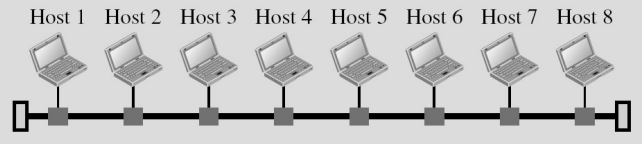
\includegraphics[scale=0.35]{images/lan-obsoleta.png}
		\caption{LAN con cavo convidiso.}
	\end{subfigure}
	\begin{subfigure}[t]{0.49 \linewidth} \centering
		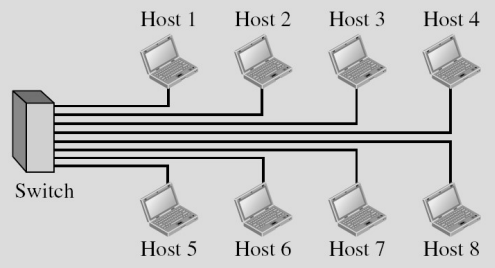
\includegraphics[scale=0.4]{images/lan-moderna.png}
		\caption{LAN con switch.}
	\end{subfigure}
	\caption{Esempi di LAN.}
	\label{fig:LAN}
\end{figure}

\begin{figure}[h!]
	\begin{subfigure}[t]{0.49 \linewidth} \centering
		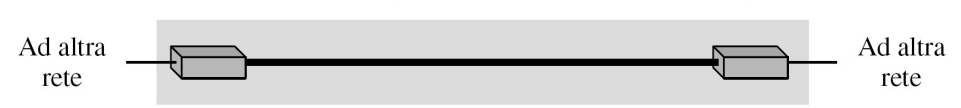
\includegraphics[width=80mm,height=10mm]{images/wan-puntopunto.png}
		\caption{WAN punto-punto.}
	\end{subfigure}
	\begin{subfigure}[t]{0.49 \linewidth} \centering
		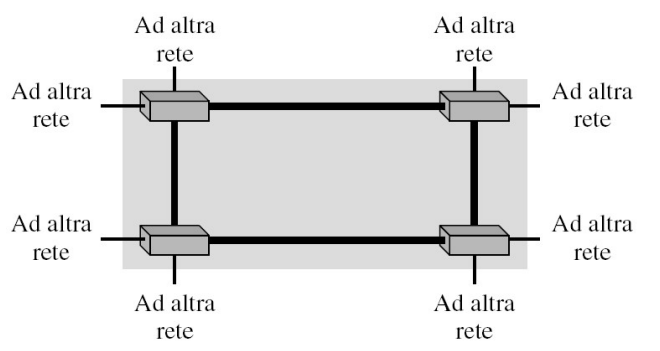
\includegraphics[scale=0.35]{images/wan-commutazione.png}
		\caption{WAN a commutazione.}
	\end{subfigure}
	\caption{Esempi di WAN.}
	\label{fig:WAN}
\end{figure}

\begin{figure}[h!]
	\begin{subfigure}[t]{0.49 \linewidth} \centering
		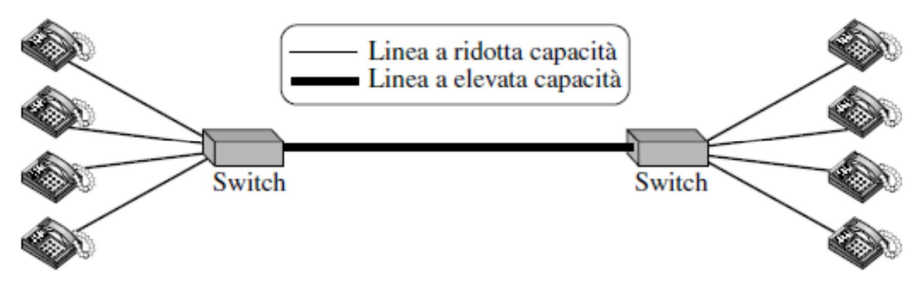
\includegraphics[scale=0.25]{images/commutazione-circuito.png}
		\caption{Rete a commutazione di circuito.}
	\end{subfigure}
	\begin{subfigure}[t]{0.49 \linewidth} \centering
		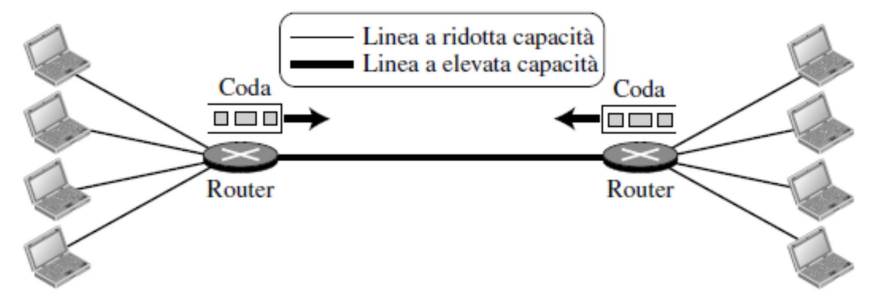
\includegraphics[scale=0.25]{images/commutazione-pacchetto.png}
		\caption{Rete a commutazione di pacchetto.}
	\end{subfigure}
	\caption{Tipi di reti.}
	\label{fig:tipi-reti}
\end{figure}

\begin{figure}[h!]
	\begin{subfigure}[t]{0.49 \linewidth} \centering
		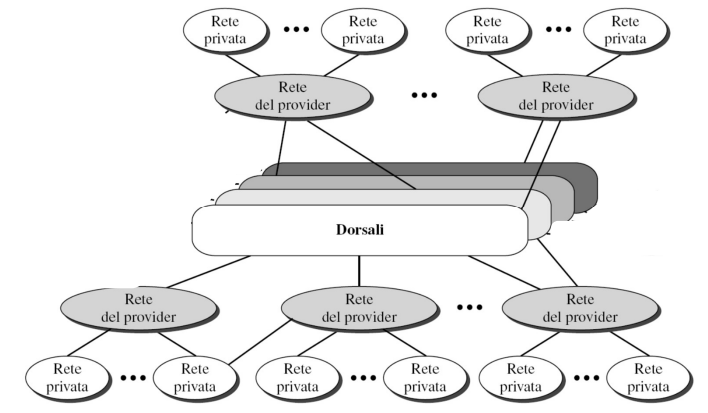
\includegraphics[scale=0.28]{images/internet-semplificata.png}
		\caption{Internet: rete di reti - versione semplificata.}
	\end{subfigure}
	\begin{subfigure}[t]{0.49 \linewidth} \centering
		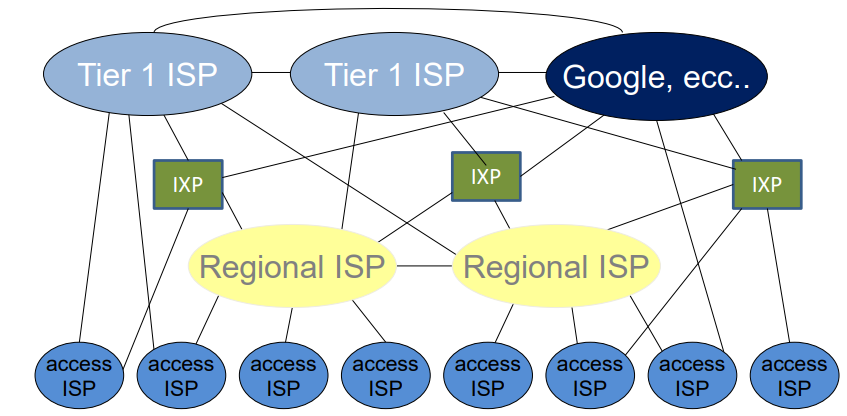
\includegraphics[scale=0.28]{images/internet-completa.png}
		\caption{Internet: rete di reti - versione moderna.}
	\end{subfigure}
	\caption{Internet.}
	\label{fig:internet}
\end{figure}

\pagebreak

\begin{figure}[h!]
	\begin{subfigure}[t]{0.49 \linewidth} \centering
		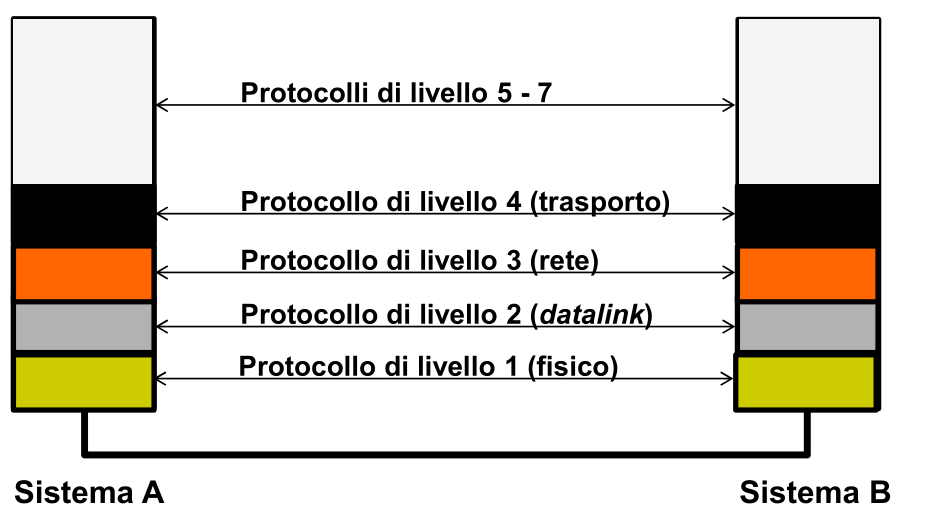
\includegraphics[scale=0.22]{images/stack-protocollare-iso_osi.png}
		\caption{Pila di protocolli.}
	\end{subfigure}
	\begin{subfigure}[t]{0.49 \linewidth} \centering
		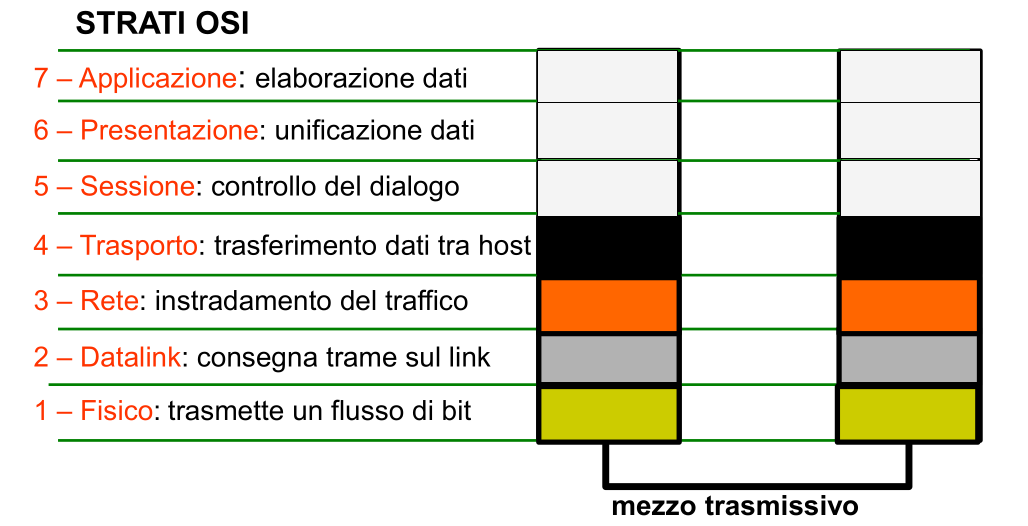
\includegraphics[scale=0.22]{images/gerarchia-layer-iso_osi.png}
		\caption{Gerarchia di strati (o "layer").}
	\end{subfigure}
	\caption{Modello ISO/OSI.}
	\label{fig:iso-osi}
\end{figure}

\begin{figure}[h!]
	\begin{subfigure}[t]{0.49 \linewidth} \centering
		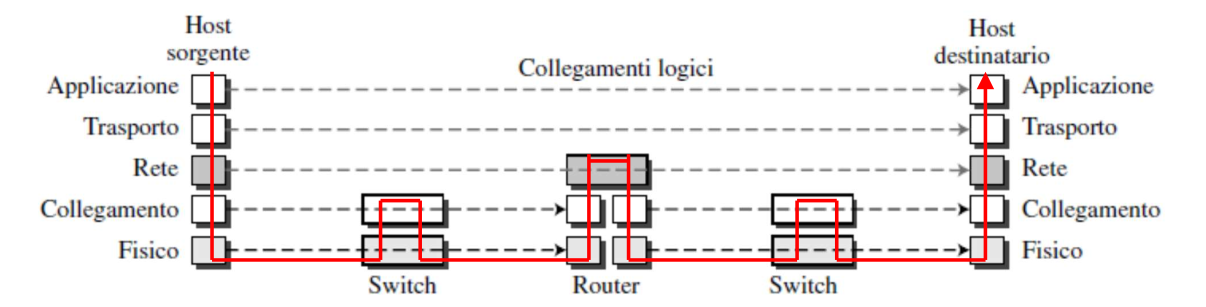
\includegraphics[scale=0.18]{images/livello-fisico-tcp_ip.png}
		\caption{Comunicazione in una internet - livello fisico.}
	\end{subfigure}
	\begin{subfigure}[t]{0.49 \linewidth} \centering
		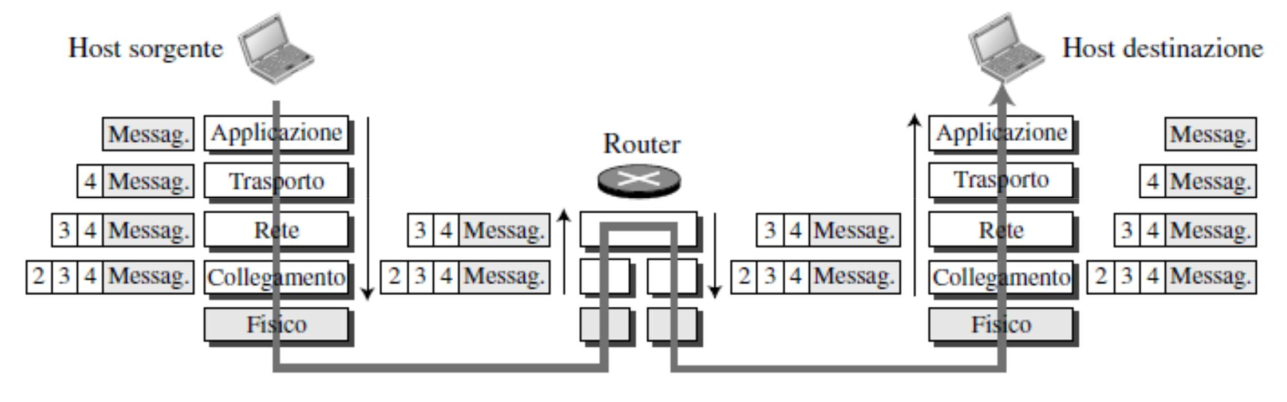
\includegraphics[scale=0.18]{images/incapsulamento-tcp_ip.png}
		\caption{Comunicazione in una internet - incapsulamento.}
	\end{subfigure}
	\caption{Comunicazione in una internet.}
	\label{fig:comunicazione-internet}
\end{figure}

\begin{figure}[h!]
	\begin{subfigure}[t]{0.49 \linewidth} \centering
		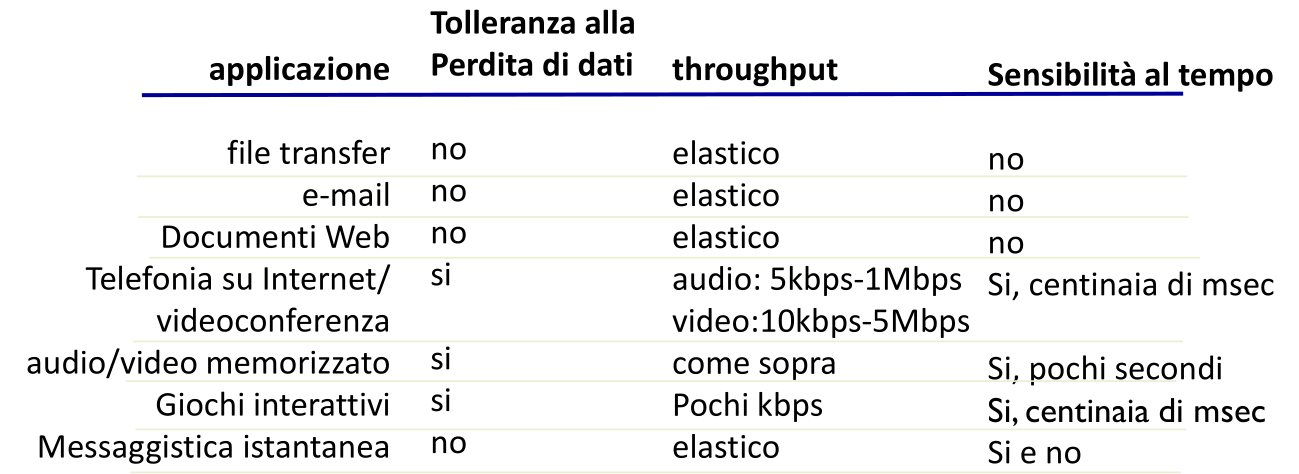
\includegraphics[scale=0.18]{images/trasporto-applicazioni-comuni.png}
		\caption{Tipo di trasporto richiesto da applicazioni comuni.}
	\end{subfigure}
	\begin{subfigure}[t]{0.49 \linewidth} \centering
		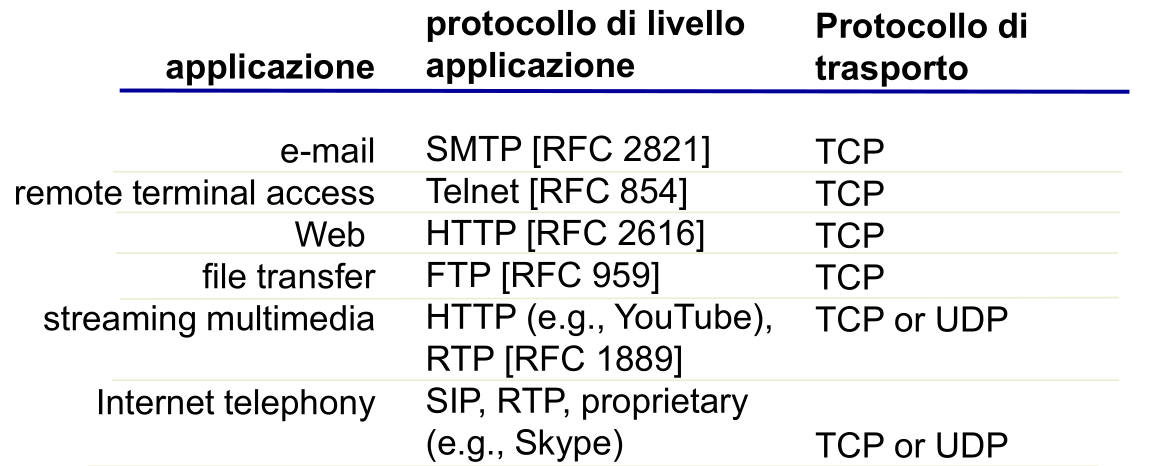
\includegraphics[scale=0.18]{images/applicazioni-internet.png}
		\caption{Esempi di applicazioni Internet e i relativi protocolli.}
	\end{subfigure}
	\caption{Esempi di applicazioni Internet.}
	\label{fig:applicazioni-internet}
\end{figure}

\begin{figure}[h!]
	\begin{subfigure}[t]{0.49 \linewidth} \centering
		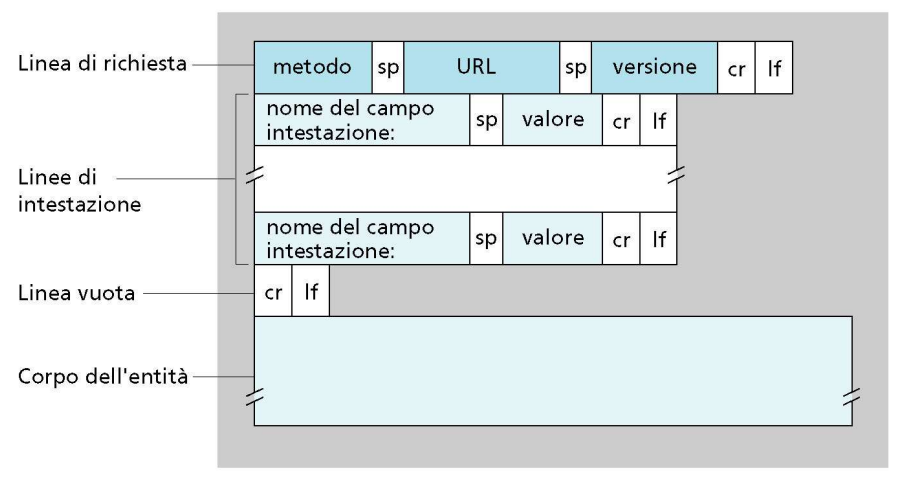
\includegraphics[scale=0.25]{images/http-request.png}
		\caption{HTTP Request Message.}
	\end{subfigure}
	\begin{subfigure}[t]{0.49 \linewidth} \centering
		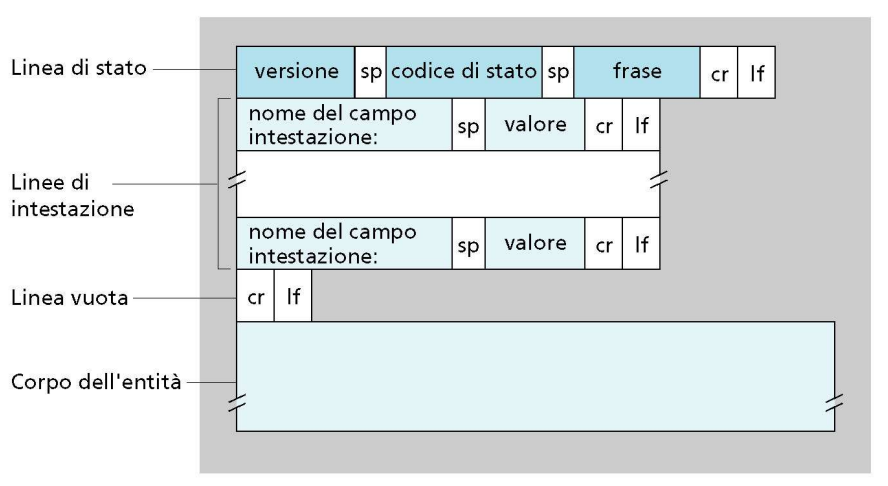
\includegraphics[scale=0.25]{images/http-response.png}
		\caption{HTTP Response Message.}
	\end{subfigure}
	\caption{Messaggi HTTP.}
	\label{fig:messaggi-http}
\end{figure}

\pagebreak

\begin{figure}[h!]
	\begin{subfigure}[t]{0.49 \linewidth} \centering
		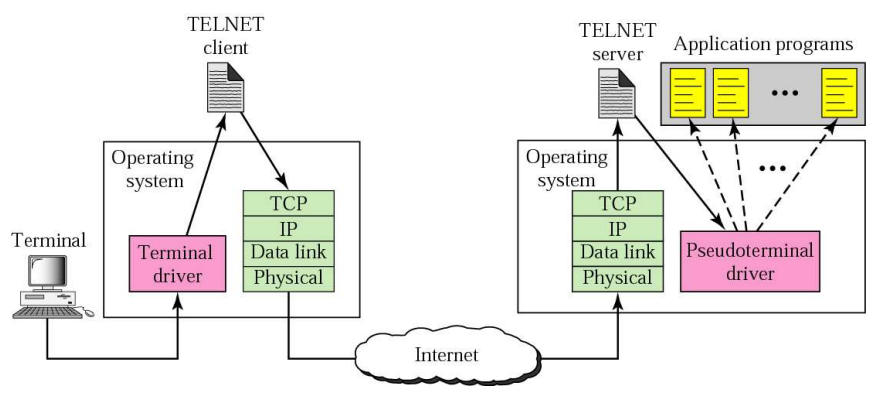
\includegraphics[scale=0.25]{images/telnet.png}
		\caption{TELNET: Login da remoto.}
	\end{subfigure}
	\begin{subfigure}[t]{0.49 \linewidth} \centering
		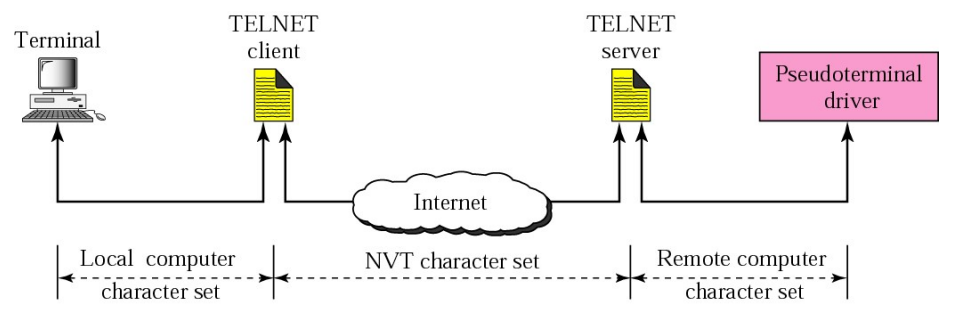
\includegraphics[scale=0.25]{images/telnet-nvt.png}
		\caption{TELNET: NVT.}
	\end{subfigure}
	\caption{TELNET.}
	\label{fig:telnet}
\end{figure}

\begin{figure}[!h]
	\begin{subfigure}[t]{0.49 \linewidth} \centering
		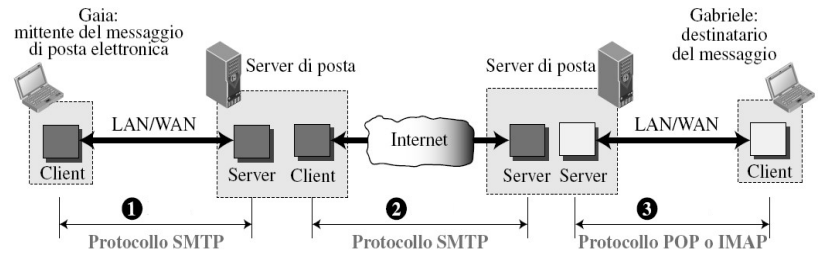
\includegraphics[scale=0.28]{images/smtp.png}
		\caption{Modello SMTP.}
	\end{subfigure}
	\begin{subfigure}[t]{0.49 \linewidth} \centering
		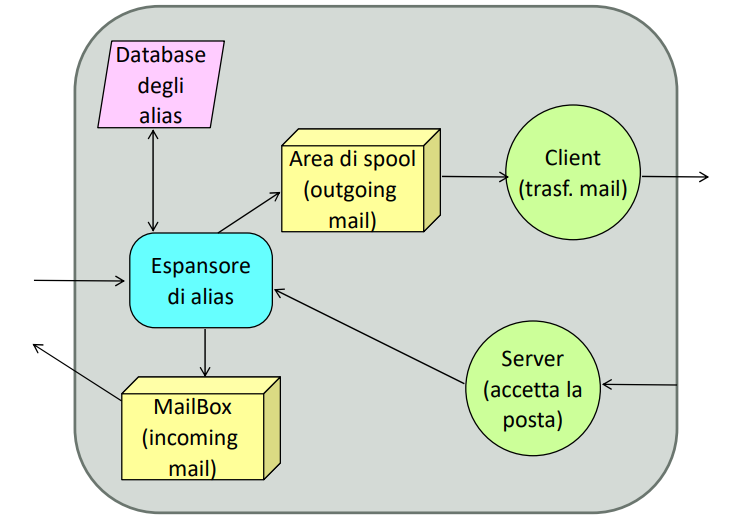
\includegraphics[scale=0.2]{images/smtp-aliasing.png}
		\caption{Server postale con gestione degli alias.}
	\end{subfigure}
	\caption{SMTP.}
	\label{fig:smtp}
\end{figure}

\begin{figure}[!h]
	\begin{subfigure}[t]{0.49 \linewidth} \centering
		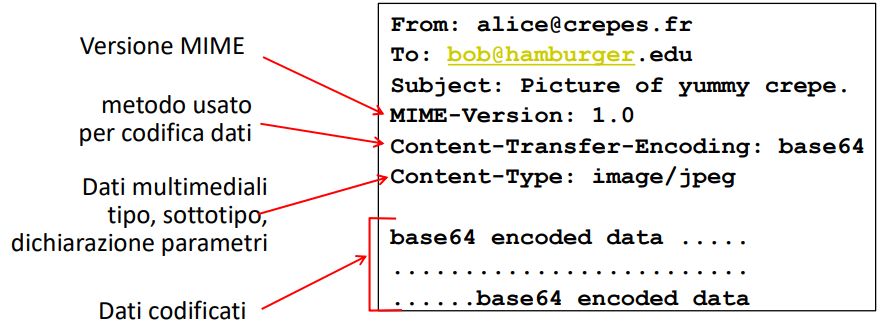
\includegraphics[scale=0.275]{images/smtp-mime.png}
		\caption{Esempio di uso del protocollo MIME.}
	\end{subfigure}
	\begin{subfigure}[t]{0.49 \linewidth} \centering
		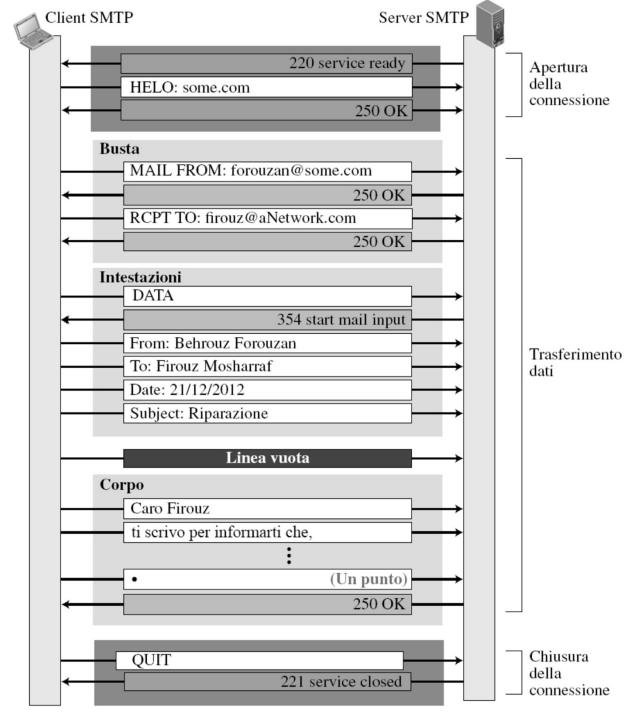
\includegraphics[scale=0.32]{images/smtp-sessione.png}
		\caption{Esempio di sessione SMTP.}
	\end{subfigure}
	\caption{SMTP: esempi di sessioni.}
	\label{fig:smtp-esempi}
\end{figure}

\pagebreak

\begin{figure}[!h]
	\centering
	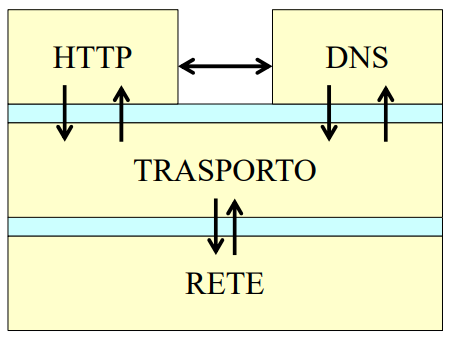
\includegraphics[scale=0.25]{images/dns-servizio.png}
	\caption{DNS: servizio di risoluzione.}
	\label{fig:dns-servizio}
\end{figure}
\begin{figure}[!h]
	\centering
	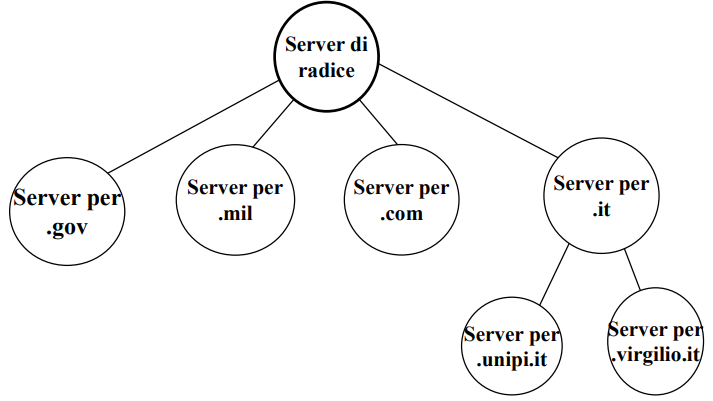
\includegraphics[scale=0.45]{images/dns-gerarchia-nameserver.png}
	\caption{Gerarchia dei name server.}
	\label{fig:dns-nameserver}
\end{figure}

\begin{figure}[!h]
	\begin{subfigure}[t]{0.49 \linewidth} \centering
		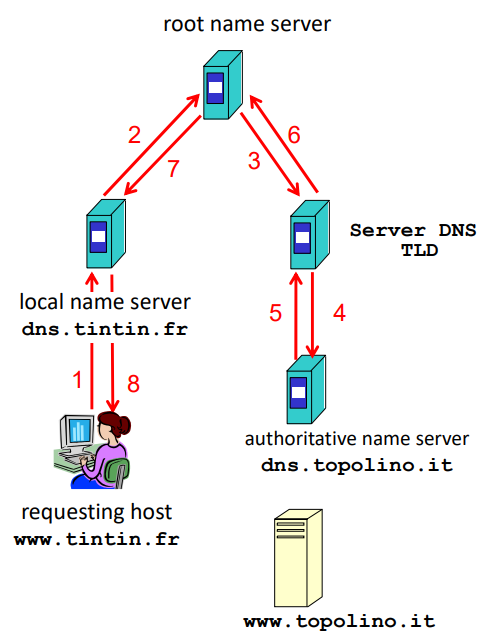
\includegraphics[scale=0.35]{images/dns-query-ricorsiva.png}
		\caption{Query DNS risolta ricorsivamente.}
	\end{subfigure}
	\begin{subfigure}[t]{0.49 \linewidth} \centering
		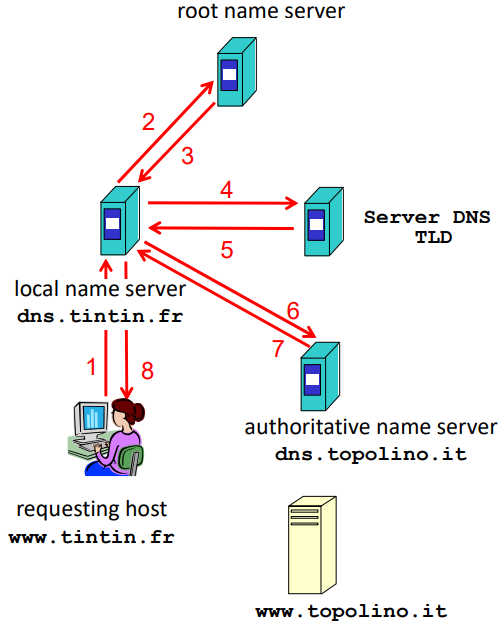
\includegraphics[scale=0.35]{images/dns-query-iterativa.png}
		\caption{Query DNS risolta iterativamente.}
	\end{subfigure}
	\caption{Query DNS.}
	\label{fig:dns-query}
\end{figure}

\pagebreak

\begin{figure}[!h]
	\centering
	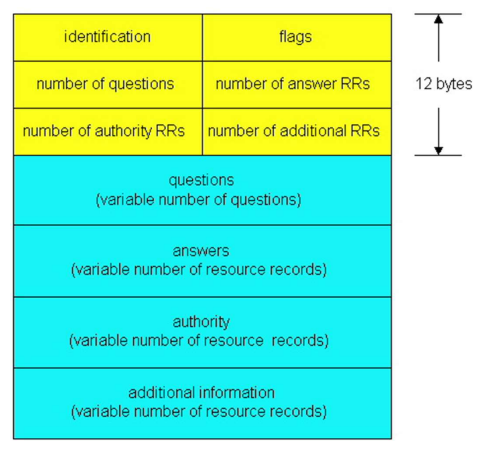
\includegraphics[scale=0.5]{images/dns-messaggio.png}
	\caption{Struttura di un messaggio DNS.}
	\label{fig:dns-messaggio}
\end{figure}
\begin{figure}[!h]
	\centering
	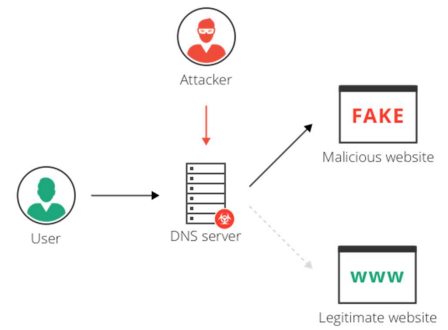
\includegraphics[scale=0.35]{images/dns-hijacking.png}
	\caption{DNS hijacking.}
	\label{fig:dns-hijacking}
\end{figure}


\begin{figure}[!h]
	\begin{subfigure}[t]{0.49 \linewidth} \centering
		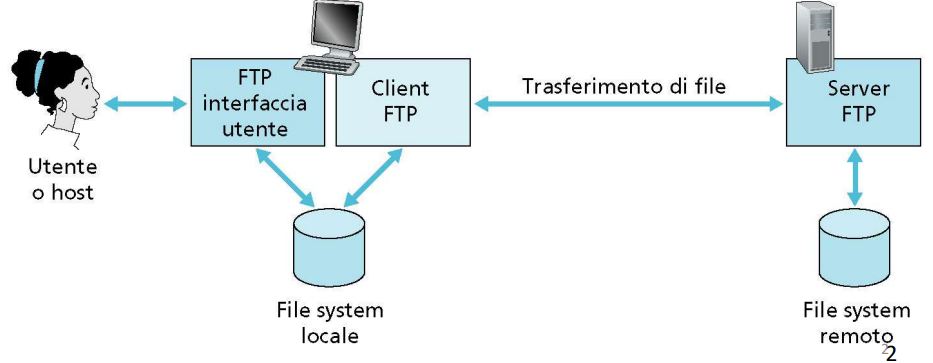
\includegraphics[scale=0.26]{images/ftp-overview.png}
		\caption{FTP: overview.}
	\end{subfigure}
	\begin{subfigure}[t]{0.49 \linewidth} \centering
		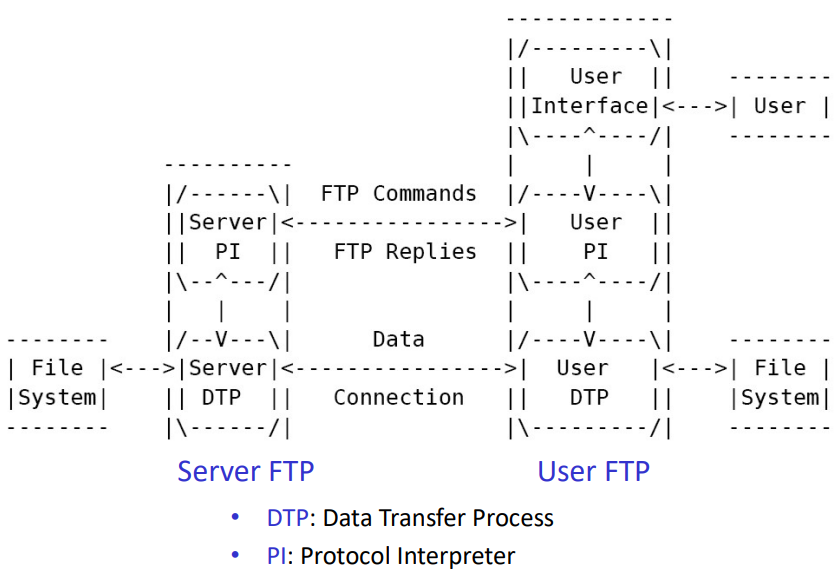
\includegraphics[scale=0.25]{images/ftp-modello.png}
		\caption{Modello FTP.}
	\end{subfigure}
	\caption{FTP.}
	\label{fig:ftp}
\end{figure}

\pagebreak

\begin{figure}[!h]
	\begin{subfigure}[t]{0.49 \linewidth} \centering
		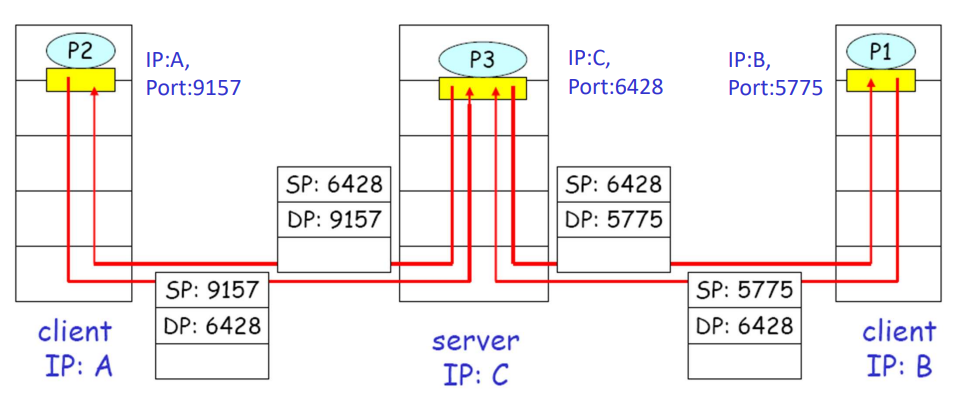
\includegraphics[scale=0.24]{images/demultiplexing-senza-connessione.png}
		\caption{Demultiplexing senza connessione.}
	\end{subfigure}
	\begin{subfigure}[t]{0.49 \linewidth} \centering
		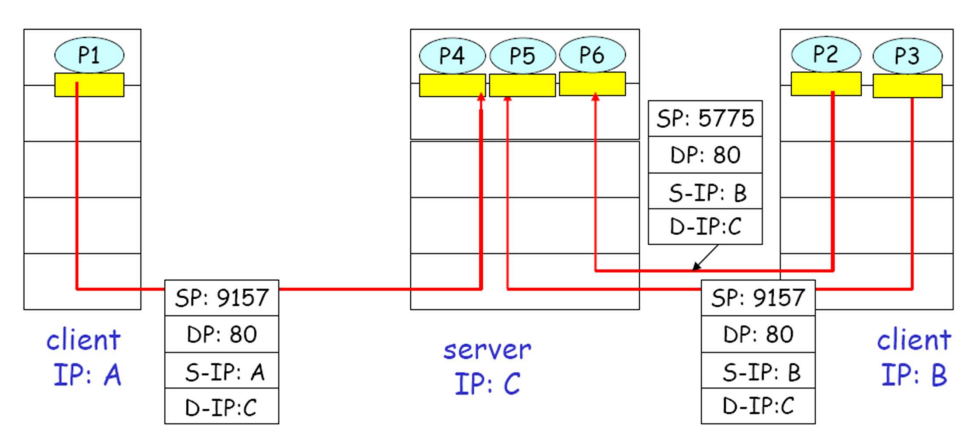
\includegraphics[scale=0.24]{images/demultiplexing-orientato-alla-connessione.png}
		\caption{Demultiplexing orientato alla connessione.}
	\end{subfigure}
	\caption{Demultiplexing.}
	\label{fig:demultiplexing}
\end{figure}

\begin{figure}[!h]
	\centering
	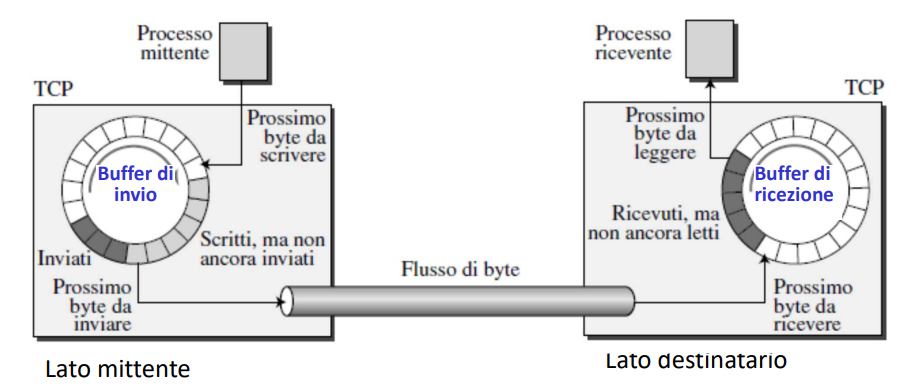
\includegraphics[scale=0.3]{images/tcp-trasferimento-bufferizzato.png}
	\caption{TCP: trasferimento bufferizzato.}
	\label{fig:tcp-trasferimento}
\end{figure}
\begin{figure}[!h]
	\centering
	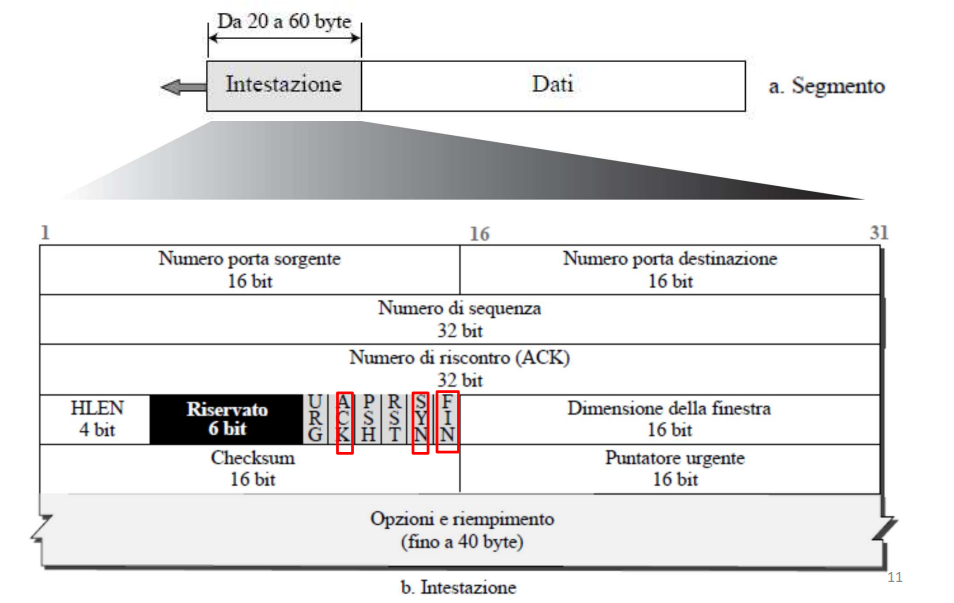
\includegraphics[scale=0.5]{images/tcp-formato-segmenti.png}
	\caption{Formato dei segmenti TCP.}
	\label{fig:tcp-segmento}
\end{figure}

\pagebreak

\begin{figure}[!h]
	\begin{subfigure}[t]{0.35 \linewidth} \centering
		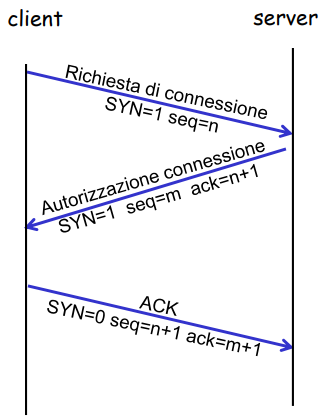
\includegraphics[scale=0.3]{images/tcp-3way-handshake-semplificato.png}
		\caption{Handshake a 3 vie: vista semplificata.}
	\end{subfigure}
	\begin{subfigure}[t]{0.64 \linewidth} \centering
		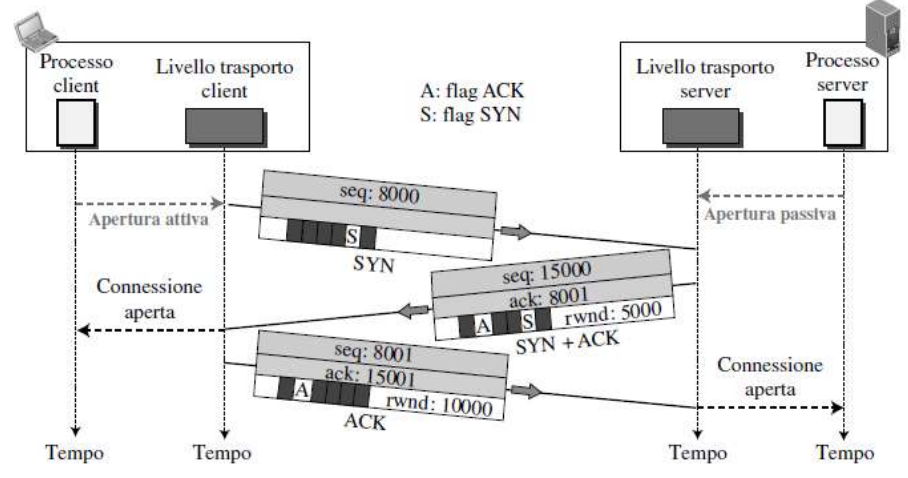
\includegraphics[scale=0.35]{images/tcp-3way-handshake.png}
		\caption{Handshake a 3 vie.}
	\end{subfigure}
	\caption{TCP: handshake.}
	\label{fig:tcp-handshake}
\end{figure}

\begin{figure}[!h]
	\centering
	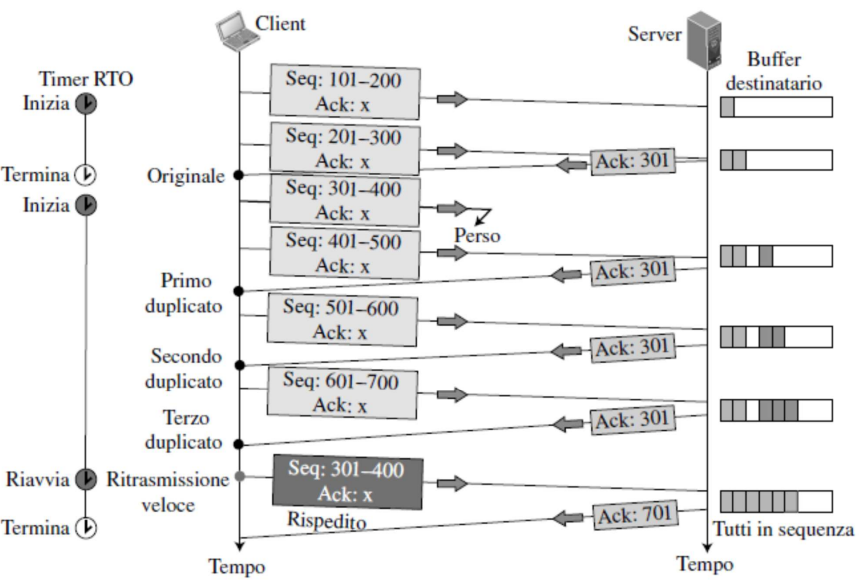
\includegraphics[scale=0.55]{images/tcp-ritrasmissione-veloce.png}
	\caption{TCP: ritrasmissione veloce.}
	\label{fig:tcp-ritrasmissione-veloce}
\end{figure}

\pagebreak

\begin{figure}[!h]
	\centering
	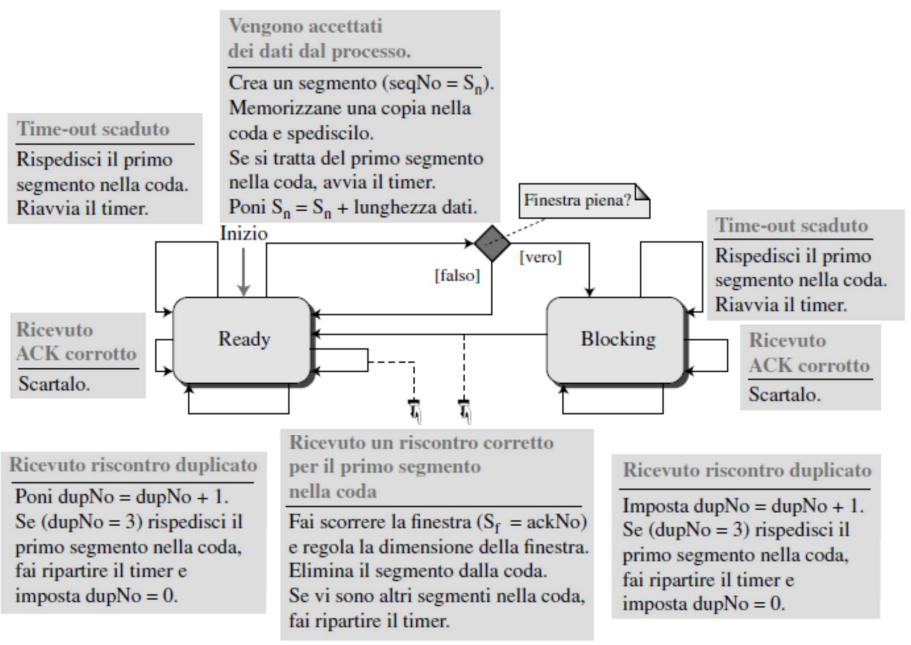
\includegraphics[scale=0.45]{images/tcp-fsm-mittente.png}
	\caption{TCP: FSM mittente.}
	\label{fig:tcp-fsm-mittente}
\end{figure}

\begin{figure}[!h]
	\centering
	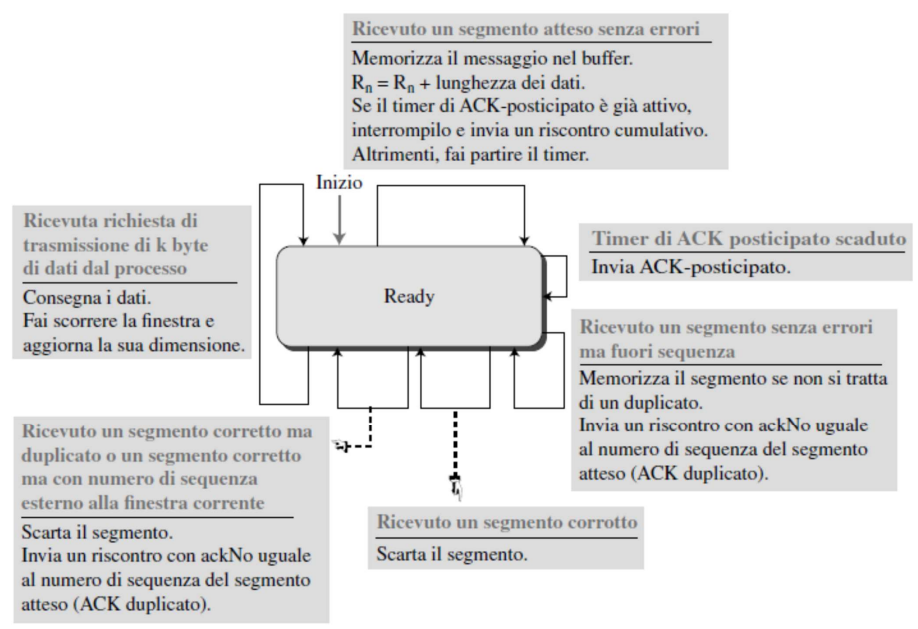
\includegraphics[scale=0.45]{images/tcp-fsm-destinatario.png}
	\caption{TCP: FSM destinatario.}
	\label{fig:tcp-fsm-destinatario}
\end{figure}

\pagebreak

\begin{figure}[!h]
	\centering
	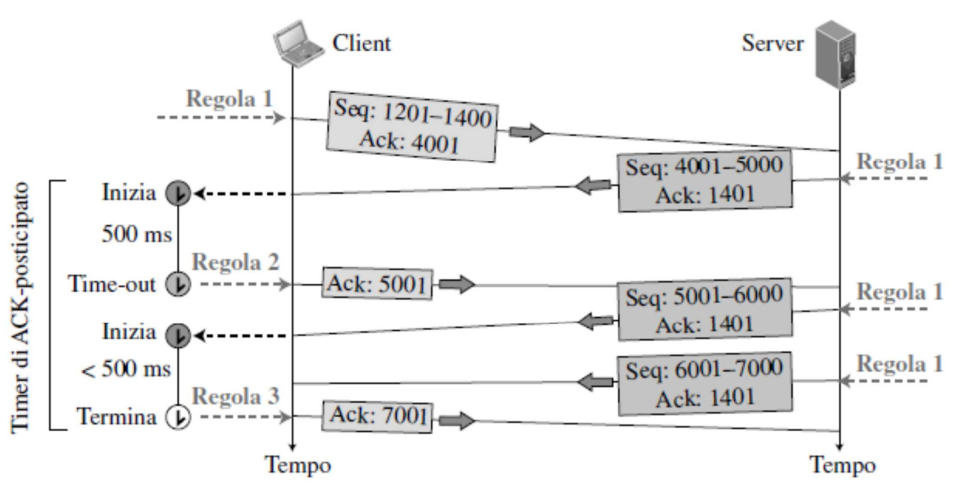
\includegraphics[scale=0.43]{images/tcp-caso-ok.png}
	\caption{TCP: operativit\`a normale.}
	\label{fig:tcp-caso-ok}
\end{figure}

\begin{figure}[!h]
	\centering
	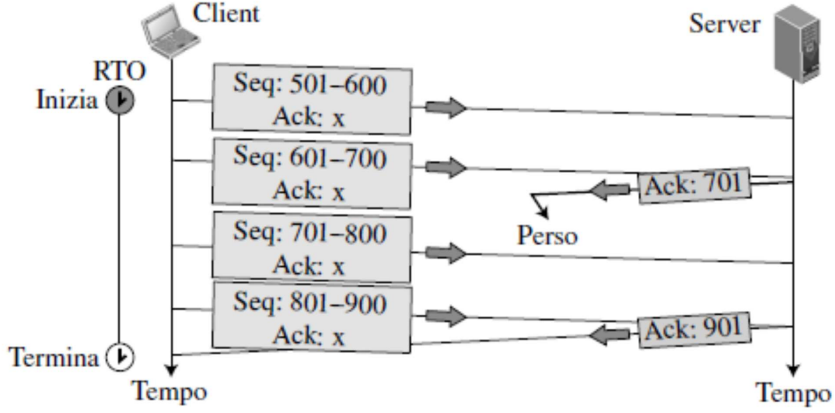
\includegraphics[scale=0.4]{images/tcp-riscontro-smarrito.png}
	\caption{TCP: riscontro smarrito.}
	\label{fig:tcp-riscontro-smarrito}
\end{figure}

\begin{figure}[!h]
	\centering
	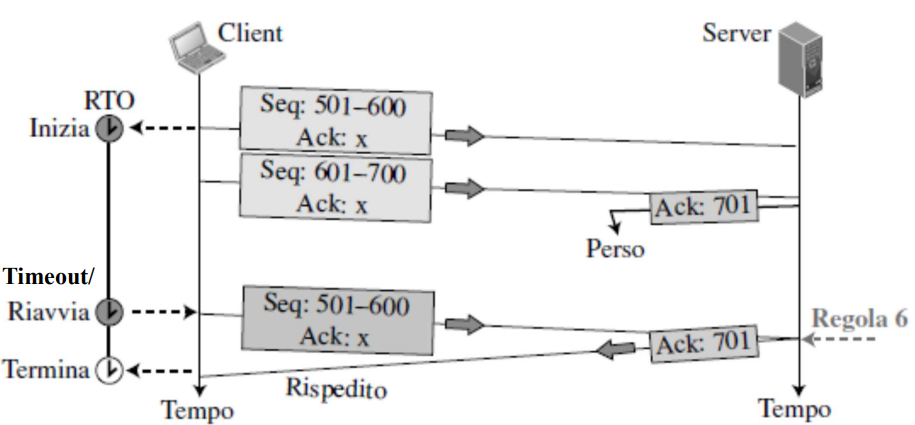
\includegraphics[scale=0.4]{images/tcp-riscontro-smarrito-ritrasmissione.png}
	\caption{TCP: riscontro smarrito corretto con ritrasmissione.}
	\label{fig:tcp-riscontro-smarrito-ritrasmissione}
\end{figure}

\pagebreak

\begin{figure}[!h]
	\centering
	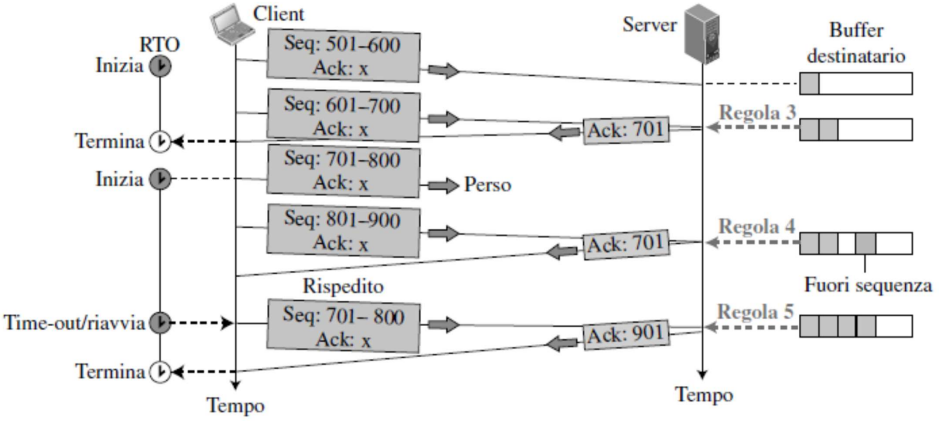
\includegraphics[scale=0.45]{images/tcp-segmento-smarrito.png}
	\caption{TCP: segmento smarrito.}
	\label{fig:tcp-segmento-smarrito}
\end{figure}

\begin{figure}[!h]
	\centering
	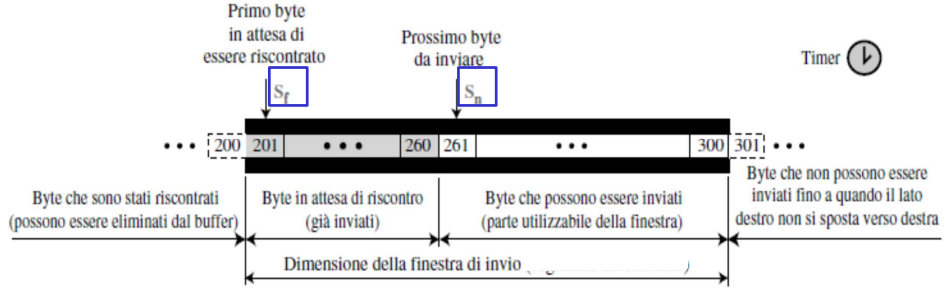
\includegraphics[scale=0.5]{images/tcp-finestra-di-trasmissione.png}
	\caption{TCP: finestra di trasmissione.}
	\label{fig:tcp-finestra-di-trasmissione}
\end{figure}

\begin{figure}[!h]
	\centering
	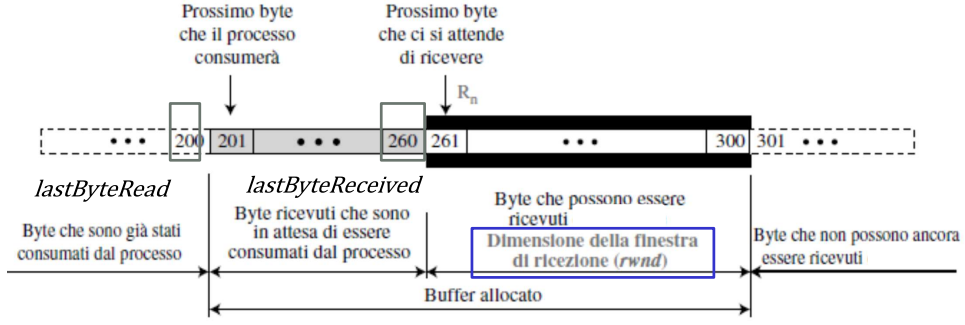
\includegraphics[scale=0.5]{images/tcp-finestra-di-ricezione.png}
	\caption{TCP: finestra di ricezione.}
	\label{fig:tcp-finestra-di-ricezione}
\end{figure}

\pagebreak

\begin{figure}[!h]
	\centering
	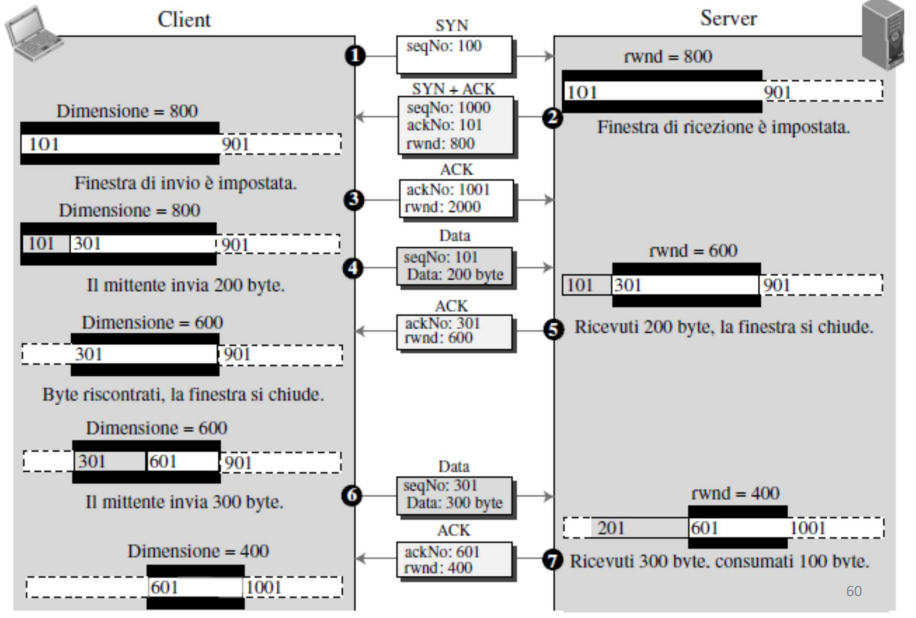
\includegraphics[scale=0.35]{images/tcp-rwnd.png}
	\caption{TCP: esempio di comunicazione con rwnd.}
	\label{fig:tcp-rwnd}
\end{figure}


\begin{figure}[!h]
	\centering
	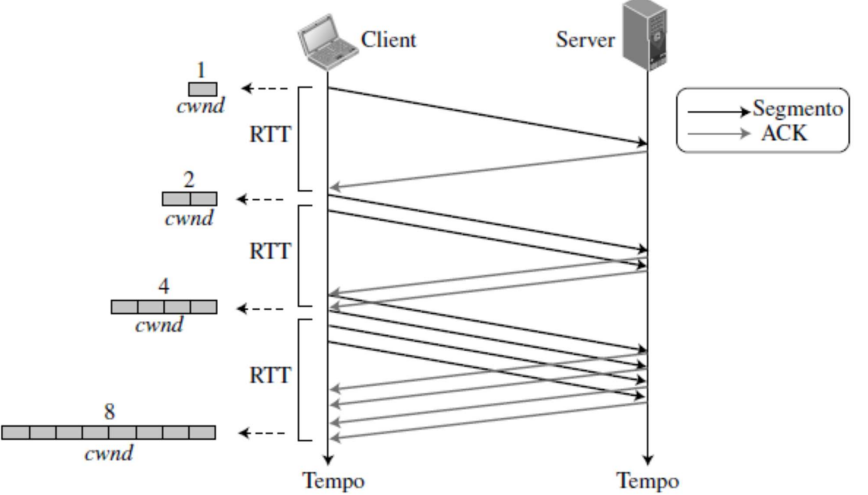
\includegraphics[scale=0.3]{images/tcp-slow-start.png}
	\caption{TCP: slow start.}
	\label{fig:tcp-slow-start}
\end{figure}


\begin{figure}[!h]
	\centering
	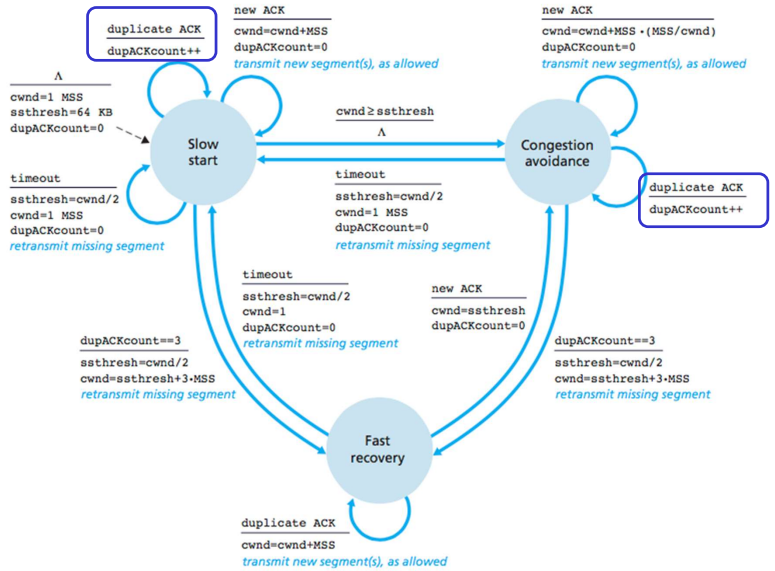
\includegraphics[scale=0.3]{images/tcp-reno-fsm.png}
	\caption{TCP Reno: macchina a stati.}
	\label{fig:tcp-reno-fsm}
\end{figure}

\pagebreak

\begin{figure}[!h]
	\centering
	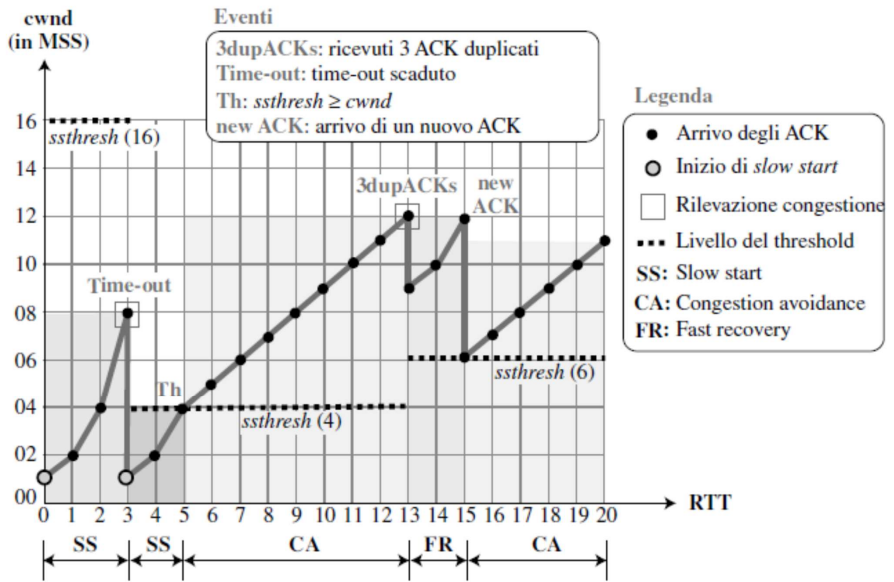
\includegraphics[scale=0.35]{images/tcp-reno-esempio.png}
	\caption{TCP Reno: esempio.}
	\label{fig:tcp-reno-esempio}
\end{figure}

\begin{figure}[!h]
	\centering
	\includegraphics[scale=0.35]{images/tcp-tahoe-fsm.png}
	\caption{TCP Tahoe: macchina a stati.}
	\label{fig:tcp-tahoe-fsm}
\end{figure}

\begin{figure}[!h]
	\centering
	\includegraphics[scale=0.35]{images/tcp-tahoe-esempio.png}
	\caption{TCP Tahoe: esempio.}
	\label{fig:tcp-tahoe-esempio}
\end{figure}

\pagebreak

\begin{figure}[!h]
	\centering
	\includegraphics[scale=0.45]{images/tcp-aimd.png}
	\caption{TCP: AIMD.}
	\label{fig:tcp-aimd}
\end{figure}

\begin{figure}[!h]
	\centering
	\includegraphics[scale=0.5]{images/tcp-half-close.png}
	\caption{TCP: half-close.}
	\label{fig:tcp-half-close}
\end{figure}

\pagebreak

\begin{figure}[!h]
	\centering
	\includegraphics[scale=0.35]{images/tcp-chiusura-3way-handshake.png}
	\caption{TCP: chiusura con handshake a 3 vie (comune nel caso di modelli client-server del tipo richiesta/risposta).}
	\label{fig:chiusura-3way}
\end{figure}

\begin{figure}[!h]
	\centering
	\includegraphics[scale=0.55]{images/tcp-apertura-chiusura.png}
	\caption{Apertura e chiusura della connessione.}
	\label{fig:tcp-apertura-chiusura}
\end{figure}

\pagebreak

\begin{figure}[!h]
	\centering
	\includegraphics[scale=0.45]{images/tcp-chiusura.png}
	\caption{Chiusura della connessione.}
	\label{fig:tcp-chiusura}
\end{figure}

\begin{figure}[!h]
	\centering
	\includegraphics[scale=0.5]{images/udp-checksum.png}
	\caption{UDP: struttura del campo checksum.}
	\label{fig:udp-checksum}
\end{figure}

\begin{figure}[!h]
	\centering
	\includegraphics[scale=0.5]{images/udp-datagramma.png}
	\caption{UDP: formato di un datagramma.}
	\label{fig:udp-datagramma}
\end{figure}

\pagebreak

\begin{figure}[!h]
	\centering
	\includegraphics[scale=0.35]{images/ip-inoltro.png}
	\caption{IP: inoltro.}
	\label{fig:ip-inoltro}
\end{figure}

\begin{figure}[!h]
	\centering
	\includegraphics[scale=0.5]{images/ip-instradamento.png}
	\caption{IP: instradamento.}
	\label{fig:ip-instradamento}
\end{figure}

\begin{figure}[!h]
	\centering
	\includegraphics[scale=0.35]{images/ip-tabella-inoltro.png}
	\caption{IP: inoltro e tabella di inoltro.}
	\label{fig:ip-tabella-inoltro}
\end{figure}

\pagebreak

\begin{figure}[!h]
	\centering
	\includegraphics[scale=0.35]{images/ip-frammentazione.png}
	\caption{IP: frammentazione.}
	\label{fig:ip-frammentazione}
\end{figure}

\begin{figure}[!h]
	\centering
	\includegraphics[scale=0.35]{images/ip-routing-decentralizzato.png}
	\caption{IP: routing decentralizzato.}
	\label{fig:ip-routing-decentralizzato}
\end{figure}

\begin{figure}[!h]
	\centering
	\includegraphics[scale=0.35]{images/ip-routing-centralizzato.png}
	\caption{IP: routing centralizzato.}
	\label{fig:ip-routing-centralizzato}
\end{figure}

\pagebreak

\begin{figure}[!h]
	\centering
	\includegraphics[scale=0.5]{images/ospf.png}
	\caption{IP: OSPF.}
	\label{fig:ospf}
\end{figure}

\begin{figure}[!h]
	\centering
	\includegraphics[scale=0.5]{images/ip-sessione-bgp.png}
	\caption{IP: sessione BGP.}
	\label{fig:ip-sessione-bgp}
\end{figure}

\pagebreak

\begin{figure}[!h]
	\centering
	\includegraphics[scale=0.5]{images/ip-datagramma.png}
	\caption{IP: formato di un datagramma.}
	\label{fig:ip-datagramma}
\end{figure}

\begin{figure}[!h]
	\centering
	\includegraphics[scale=0.5]{images/ip-classless-addressing.png}
	\caption{IP: indirizzamento senza classi.}
	\label{fig:ip-classless-addressing}
\end{figure}

\pagebreak

\begin{figure}[!h]
	\centering
	\includegraphics[scale=0.5]{images/ip-tabella-nat.png}
	\caption{IP: tabella di traduzione NAT.}
	\label{fig:ip-nat}
\end{figure}

\begin{figure}[!h]
	\centering
	\includegraphics[scale=0.5]{images/dhcp-esempio.png}
	\caption{DHCP: esempio di sessione.}
	\label{fig:dhcp-esempio}
\end{figure}

\pagebreak

\begin{figure}[!h]
	\centering
	\includegraphics[scale=0.35]{images/routers-struttura.png}
	\caption{Router: struttura.}
	\label{fig:routers-struttura}
\end{figure}

\begin{figure}[!h]
	\begin{subfigure}[t]{0.32 \linewidth} \centering
		\includegraphics[scale=0.45]{images/switching-fabric-memory.png}
		\caption{Switching fabric: memory.}
	\end{subfigure}
	\begin{subfigure}[t]{0.32 \linewidth} \centering
		\includegraphics[scale=0.45]{images/switching-fabric-bus.png}
		\caption{Switching fabric: bus.}
	\end{subfigure}
	\begin{subfigure}[t]{0.32 \linewidth} \centering
		\includegraphics[scale=0.45]{images/switching-fabric-crossbar.png}
		\caption{Switching fabric: crossbar.}
	\end{subfigure}
	\caption{Router: switching fabric.}
	\label{fig:switching-fabric}
\end{figure}

\begin{figure}[!h]
	\centering
	\includegraphics[scale=0.4]{images/ip-tunneling.png}
	\caption{IP: IPv4-to-IPv6 tunneling.}
	\label{fig:ip-tunneling}
\end{figure}

\pagebreak

\begin{figure}[!h]
	\centering
	\includegraphics[scale=0.5]{images/ipv6-messaggio.png}
	\caption{IPv6: formato di un messaggio.}
	\label{fig:ipv6-messaggio}
\end{figure}

\end{sloppypar}
\end{document}